%%%%%%%%%%%%%%%%%%%%%%%%%%%%%%%%%%%%%%%%%%%%%%%%%%%%%%%%%%%%%%%%%%%%%%%%%%%%%%%%
%
% Template license:
% CC BY-NC-SA 3.0 (http://creativecommons.org/licenses/by-nc-sa/3.0/)
%
%%%%%%%%%%%%%%%%%%%%%%%%%%%%%%%%%%%%%%%%%%%%%%%%%%%%%%%%%%%%%%%%%%%%%%%%%%%%%%%%

%----------------------------------------------------------------------------------------
%	PACKAGES AND OTHER DOCUMENT CONFIGURATIONS
%----------------------------------------------------------------------------------------

\documentclass[
11pt, % The default document font size, options: 10pt, 11pt, 12pt
%oneside, % Two side (alternating margins) for binding by default, uncomment to switch to one side
%chapterinoneline,% Have the chapter title next to the number in one single line
spanish,
singlespacing, % Single line spacing, alternatives: onehalfspacing or doublespacing
%draft, % Uncomment to enable draft mode (no pictures, no links, overfull hboxes indicated)
%nolistspacing, % If the document is onehalfspacing or doublespacing, uncomment this to set spacing in lists to single
%liststotoc, % Uncomment to add the list of figures/tables/etc to the table of contents
%toctotoc, % Uncomment to add the main table of contents to the table of contents
parskip, % Uncomment to add space between paragraphs
%codirector, % Uncomment to add a codirector to the title page
headsepline, % Uncomment to get a line under the header
]{MastersDoctoralThesis} % The class file specifying the document structure



%----------------------------------------------------------------------------------------
%	INFORMACIÓN DE LA MEMORIA
%----------------------------------------------------------------------------------------

\thesistitle{Sistema de gestión de alertas y tareas de procesos de planta - Control de acceso} % El títulos de la memoria, se usa en la carátula y se puede usar el cualquier lugar del documento con el comando \ttitle

% Nombre del posgrado, se usa en la carátula y se puede usar el cualquier lugar del documento con el comando \degreename
%\posgrado{Carrera de Especialización en Sistemas Embebidos} 
\posgrado{Carrera de Especialización en Internet de las Cosas} 
%\posgrado{Carrera de Especialización en Intelegencia Artificial}
%\posgrado{Maestría en Sistemas Embebidos} 
%\posgrado{Maestría en Internet de las cosas}

\author{Lionel Gutierrez} % Tu nombre, se usa en la carátula y se puede usar el cualquier lugar del documento con el comando \authorname

\director{Gustavo Ramoscelli (UNS)} % El nombre del director, se usa en la carátula y se puede usar el cualquier lugar del documento con el comando \dirname
\codirector{Nombre del codirector (pertenencia)} % El nombre del codirector si lo hubiera, se usa en la carátula y se puede usar el cualquier lugar del documento con el comando \codirname.  Para activar este campo se debe descomentar la opción "codirector" en el comando \documentclass, línea 23.

\juradoUNO{José Alamos (pertenencia)} % Nombre y pertenencia del un jurado se usa en la carátula y se puede usar el cualquier lugar del documento con el comando \jur1name
\juradoDOS{Leandro Lanzieri Rodriguez (pertenencia)} % Nombre y pertenencia del un jurado se usa en la carátula y se puede usar el cualquier lugar del documento con el comando \jur2name
\juradoTRES{Leopoldo Zimperz (pertenencia)} % Nombre y pertenencia del un jurado se usa en la carátula y se puede usar el cualquier lugar del documento con el comando \jur3name

%\ciudad{Ciudad Autónoma de Buenos Aires}
\ciudad{ciudad de Villa Mercedes}

\fechaINICIO{marzo de 2020}
\fechaFINAL{marzo de 2021}


\keywords{Sistemas embebidos, FIUBA} % Keywords for your thesis, print it elsewhere with \keywordnames


\begin{document}


\frontmatter % Use roman page numbering style (i, ii, iii, iv...) for the pre-content pages

\pagestyle{plain} % Default to the plain heading style until the thesis style is called for the body content


%----------------------------------------------------------------------------------------
%	RESUMEN - ABSTRACT 
%----------------------------------------------------------------------------------------

\begin{abstract}
\addchaptertocentry{\abstractname} % Add the abstract to the table of contents
%
%The Thesis Abstract is written here (and usually kept to just this page). The page is kept centered vertically so can expand into the blank space above the title too\ldots
\centering

La presente memoria describe el diseño e implementación de un sistema de control de acceso de personal de terceros a una locación industrial. El sistema garantiza que solo aquellas personas que tienen en regla los requisitos legales y médicos solicitados accedan, evitando que la empresa sea responsable ante posibles accidentes o incidentes de dicho personal. El trabajo desarrollado es la primera etapa de un proyecto integral de gestión de alertas y procesos para la empresa Tenaris Metalmecánica, sobre el cual se agregarán a futuro nuevos casos de uso.

Para la elaboración del trabajo se aplicaron conocimientos adquiridos a lo largo de la carrera, principalmente los referidos a gestión de proyectos, desarrollo de aplicaciones web y multiplataforma, protocolos de Internet y seguridad en IoT. Además, se integraron tecnologías de base de datos relacionales y no relacionales y se aplicaron varias técnicas de testing.

\end{abstract}

%----------------------------------------------------------------------------------------
%	CONTENIDO DE LA MEMORIA  - AGRADECIMIENTOS
%----------------------------------------------------------------------------------------

\begin{acknowledgements}
%\addchaptertocentry{\acknowledgementname} % Descomentando esta línea se puede agregar los agradecimientos al índice
\vspace{1.5cm}

AGREGAR AGRADECIMIENTO

\end{acknowledgements}

%----------------------------------------------------------------------------------------
%	LISTA DE CONTENIDOS/FIGURAS/TABLAS
%----------------------------------------------------------------------------------------

\tableofcontents % Prints the main table of contents

\listoffigures % Prints the list of figures

\listoftables % Prints the list of tables


%----------------------------------------------------------------------------------------
%	CONTENIDO DE LA MEMORIA  - DEDICATORIA
%----------------------------------------------------------------------------------------

%\dedicatory{\textbf{Dedicado a... [OPCIONAL]}}  % escribir acá si se desea una dedicatoria

%----------------------------------------------------------------------------------------
%	CONTENIDO DE LA MEMORIA  - CAPÍTULOS
%----------------------------------------------------------------------------------------

\mainmatter % Begin numeric (1,2,3...) page numbering

\pagestyle{thesis} % Return the page headers back to the "thesis" style

% Incluir los capítulos como archivos separados desde la carpeta Chapters

% Chapter 1

\chapter{Introducción general} % Main chapter title

\label{Chapter1} % For referencing the chapter elsewhere, use \ref{Chapter1} 
\label{IntroGeneral}

En el presente capítulo se describen los diferentes métodos de control de acceso en el ámbito de Internet de las Cosas (IoT) y se exponen la motivación, los objetivos y el alcance del trabajo.

%----------------------------------------------------------------------------------------

% Define some commands to keep the formatting separated from the content 
\newcommand{\keyword}[1]{\textbf{#1}}
\newcommand{\tabhead}[1]{\textbf{#1}}
\newcommand{\code}[1]{\texttt{#1}}
\newcommand{\file}[1]{\texttt{\bfseries#1}}
\newcommand{\option}[1]{\texttt{\itshape#1}}
\newcommand{\grados}{$^{\circ}$}

%----------------------------------------------------------------------------------------

%\section{Introducción}

%----------------------------------------------------------------------------------------
\section{Estado del arte}

En esta sección se realiza una introducción a las soluciones IoT y su uso para gestionar el control de acceso en las empresas.

\subsection{Tecnología IoT}

Con la expansión de Internet y las tecnologías de conectividad móvil 3G, 4G y el advenimiento del 5G, se ha producido una revolución en el acceso a la información con un fuerte impacto en la educación, el modo de comunicarnos, las empresas, la ciencia, el gobierno y la humanidad en general. En este contexto, Internet de las Cosas representa la próxima revolución de Internet, dado que su desarrollo está permitiendo dar un gran salto en la capacidad de
reunir, analizar y distribuir datos, convirtiéndolos en información, conocimiento, y en última instancia, sabiduría \citep{WEBSITE:IOT}.

Este término que fue propuesto en 1999, por Kevin Ashton, en el Auto-ID Center del MIT, en donde se realizaban investigaciones sobre RFID y tecnologías de sensores \citep{WEBSITE:IOTMIT}. Es un concepto que refiere a la interconexión digital de objetos cotidianos con Internet \citep{WEBSITE:IOTDefinicion}. Según la definición del Grupo de soluciones empresariales basadas en Internet (IBSG, Internet Business Solutions Group) de Cisco, IoT es sencillamente el punto en el tiempo en el que se conectaron a Internet más ``cosas u objetos'' que personas.

En ese sentido, en 2003 había aproximadamente 6,3 mil millones de personas en el planeta, y 500 millones de dispositivos conectados a Internet. Si dividimos la cantidad de dispositivos conectados por la población mundial de entonces, el resultado era de menos de un dispositivo (0,08) por persona. Mientras que el crecimiento exponencial de los teléfonos inteligentes y las tablets llevó a que en 2010 se elevara a 12,5 mil millones la cantidad de dispositivos conectados a Internet, en tanto la población mundial ascendió a 6,8 mil millones. Tal relación arroja como resultado que el número de dispositivos conectados por persona pasó a ser superior a 1 (1,84 para ser exactos) por primera vez en la historia. En esta línea, se prevé que para el 2025 tendremos alrededor de 41.600 millones de dispositivos conectados \citep{WEBSITE:IOTFechas}.

Conforme lo desarrollado en los párrafos anteriores, IoT se trata principalmente de una red de interconexión digital entre objetos, personas e Internet, que permite el intercambio de datos con otros dispositivos. Esto hace que se pueda capturar información clave sobre el uso y el rendimiento de objetos para así detectar patrones, hacer recomendaciones, mejorar la eficiencia y crear experiencias únicas para los usuarios. En definitiva, esta tecnología está transformando la vida de las personas. Algunos ejemplos son impactantes. Tal es el caso de los pacientes que ingieren dispositivos que
al ingresar a sus cuerpos ayudan a los médicos a diagnosticar y determinar las causas de ciertas enfermedades. También es posible colocar sensores pequeñísimos conectados a Internet en plantas, animales y fenómenos geológicos para medirlos, estudiarlos y prever sus comportamientos. En la figura \ref{fig:Iot} se muestra un diagrama donde se ven las interconexiones de IoT entre dispositivos y los elementos asociados.

\begin{figure}[ht]
	\centering
	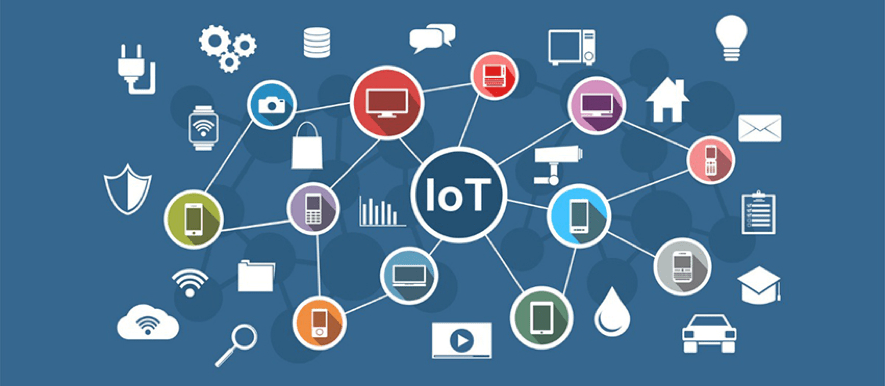
\includegraphics[width=1\textwidth]{./Figures/iot.png}
	\caption{Interconexión de dispositivos y tecnologías en IoT.}
	\label{fig:Iot}
\end{figure}

Resulta importante destacar que existe una correlación directa entre los datos y la sabiduría. Cuántos más datos se generan, más conocimiento y sabiduría pueden obtener las personas. IoT aumenta drásticamente la cantidad de datos que están disponibles para que los procesemos. Este aumento, combinado con la capacidad de Internet de comunicarlos, hará posible que las personas acumulen saberes valiosos. En la figura \ref{fig:Sabiduria} se muestra un diagrama de la correlación entre datos y sabiduría.

\begin{figure}[ht]
	\centering
	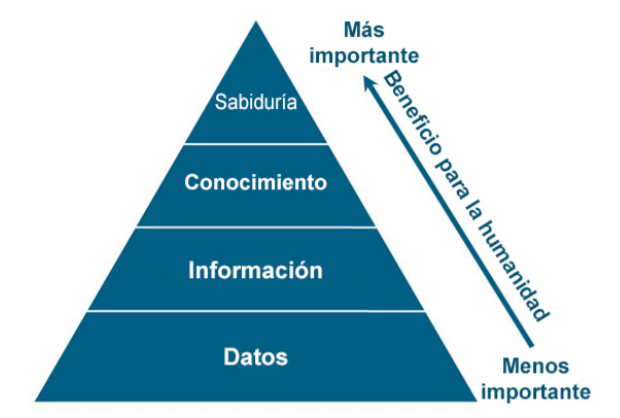
\includegraphics[width=1\textwidth]{./Figures/sabiduria.png}
	\caption{Correlación entre datos y sabiduría.}
	\label{fig:Sabiduria}
\end{figure}

En lo que respecta a las empresas, con el surgimiento de IoT aparece el fenómeno de la transformación digital, que consiste en la aplicación de la tecnología digital para generar un entorno adecuado que facilite la innovación de las empresas y la industria. En este contexto, el desarrollo de nuestro trabajo propone realizar una transformación digital en la empresa Tenaris Metalmecánica, aprovechando estas tecnologías disruptivas.

\subsection{Control de acceso}

El control de acceso se refiere a los mecanismos que permiten o restringen la entrada de una persona o vehículo a una empresa o recinto, mediante su identificación. Dentro de los principales objetivos del control de acceso se incluye el de garantizar la seguridad y facilitar la organización empresarial. Cuando una organización instala un sistema de control de acceso, lo hace básicamente pensando en tres propósitos:

\begin{itemize}
\item Cuidar de la integridad física de las personas.
\item Proteger la información de la compañía (bases de datos, material sensible, etc.).
\item Custodiar los activos de la empresa.
\end{itemize}

Para cumplir con tales propósitos, se emplean diferentes medios para monitorear y controlar el acceso de las personas a una instalación. Décadas atrás se usaban sistemas de cerraduras y llaves. Dicho método, además de ser vulnerable, representaba gastos adicionales para la empresa ante el robo o extravío. Con el advenimiento de Internet, y principalmente de IoT, el control de acceso migró a sistemas más robustos con credenciales electrónicas o identificación biométrica.

\subsubsection{Factores de autenticación}
Para un proceso de identificación, sea físico o digital, se debe comprobar la identidad de la persona que hace la solicitud. Esa verificación se puede realizar usando uno o varios factores de autenticación. Los factores de autenticación se pueden dividir en:

\begin{itemize}
\item Lo que sé: el conocimiento que la persona tiene, puede ser un PIN, una contraseña o un patrón.
\item Lo que tengo: la identificación que posee un individuo para certificar que es él, como una credencial física o virtual.
\item Lo que soy: los rasgos corporales únicos de la persona que se utilizan para verificar la identidad (biometría).
\end{itemize}

Para aumentar el nivel de seguridad, los sistemas modernos implementan varios factores de autenticación en los puntos de acceso, combinando ``lo que tengo'' con ``lo que sé'' y con ``lo que soy'' \citep{WEBSITE:ControlAcceso}.

\subsubsection{Clasificación de sistemas de control de acceso}

Los sistemas de control de acceso para personas se clasifican por dos criterios: conectividad y método de identificación \citep{WEBSITE:ControlAccesoPersonas}.

Por su conectividad:

\begin{itemize}
\item Controles de acceso autónomos: no necesitan conectarse a la red y no guardan datos de los movimientos que producen, sino que se limitan a abrir las puertas o barreras. 
\item Controles de acceso conectados en red: éstos, además de permitir los accesos, registran las entradas y salidas de personas. Deben conectarse a Internet, ya que la información sobre tales movimientos se descarga en una aplicación para poder generar informes.
\end{itemize}

Por su método de identificación:

\begin{itemize}
\item Biométricos: La identificación se produce mediante la lectura de datos físicos individuales que imposibilitan la suplantación al ser intransferibles, por lo que se consideran los sistemas más seguros. Su empleo implica el cumplimiento de normativas en materia de protección de datos y no están permitidos en todas las empresas. Dentro de este grupo tenemos los métodos de reconocimiento facial y huella dactilar.
\item Tarjetas: En muchas oficinas y en otros lugares de trabajo como laboratorios, talleres o fábricas, donde se realizan tareas manuales y por cuestiones de higiene, no se aconseja utilizar la huella dactilar y se emplean, en cambio, llaveros y tarjetas. Estas últimas son de dos clases:
	\begin{itemize}
	\item Tarjetas magnéticas: tienen una banda magnética que contiene los datos de cada persona y se introduce en el lector para solicitar el acceso.
	\item Tarjetas (RFID): utilizan radiofrecuencia y no requieren contacto con el lector para activar el mecanismo que abre la cerradura. Por tal motivo se llaman ``tarjetas de proximidad''.
	\end{itemize}
\item Contraseña numérica: algunos sistemas de control de accesos permiten fichar poniendo una contraseña en el teclado del propio terminal.
\end{itemize}

\subsubsection{Estudio de mercado}

Para nuestro trabajo se realizó un análisis de los sistemas existentes en el mercado y se encontró que la seguridad y confiabilidad de las soluciones existentes van en relación a su precio. Se detectó que la gran mayoría de los sistemas del mercado son cerrados y auto-gestionados, lo que limita su integración con otros sistemas. Dicha limitación atenta contra el valor agregado propuesto en este proyecto.

Por otro lado, si bien existen productos que pueden integrarse con asistentes de voz, como Echo o Alexa de Amazon o Home de Google, en nuestro caso se desaconseja su uso, puesto que éstos recolectan datos sensibles que atentan contra la política de privacidad empresarial. También hay sistemas que permiten el acceso mediante huella, lo cual puede resultar muy cómodo, pero no es útil en la locación industrial donde se va a implementar el trabajo, ya que se requiere una política especial para el guardado de los datos y no divulgación de las huellas dactilares. 

En el capítulo 4, en la sección \ref{sec:comparativa} se realiza un análisis comparativo de las soluciones estudiadas y las ventajas y desventajas en relación con el trabajo desarrollado. En particular se analizaron dos soluciones, una de Pronext (Pronext KY800 \citep{WEBSITE:Ponext}) y una de Samsung (Samsung SHS-H505 \citep{WEBSITE:Samsung}). Si bien dichas soluciones no son costosas y brindan algunas características interesantes como doble factor de autenticación
o acceso mediante huella, no soportan conexión con sistemas externos. Dicha situación no permite el agregado de valor a los datos recolectados y su trasformación en información valiosa para la toma de decisiones.


%----------------------------------------------------------------------------------------

\section{Motivación}

La empresa Tenaris Metalmecánica cuenta con una planta industrial que elabora varillas de bombeo para la extracción de petróleo. Para ello, en sus procesos productivos utiliza servicios de terceros a fin de implementar mejoras en éstos y realizar obras civiles y mecánicas. Todo personal externo que ingresa a la planta debe cumplir un conjunto de requisitos legales y médicos. De este modo, si sucede algún incidente o accidente, la empresa está cubierta y evita problemas legales. Durante el último año se detectaron en auditorías internas varios eventos de ingresos de usuarios con documentación vencida. Por lo tanto, se necesita actuar con celeridad e implementar un sistema de control que detecte y bloquee estos accesos indebidos.

Adicionalmente, ante la necesidad de mejorar la calidad de los productos manufacturados a clientes, se requiere contar con alertas tempranas ante desvíos en los diferentes procesos industriales y de soporte de la empresa. En tal sentido, se han identificado problemas recurrentes que son planteados en reuniones diarias de gestión, pero que quedan sin solución por no ser abordados sistemáticamente. Estas dificultades han derivado en no conformidades de calidad, pérdida de dinero para la empresa y tiempo de recursos humanos valiosos. Por lo tanto, se requiere generar, conjuntamente al sistema de control de terceros, un sistema integral de gestión de alertas que permita activar diferentes tipos de actuadores y adaptarse a distintos casos de uso que se irán agregando en sucesivas etapas. 

En esta primera instancia y para el trabajo proyectado, el objetivo será controlar los ingresos de terceros a la planta y sentar las bases para poder implementar a futuro el sistema de gestión integral mencionado.

%----------------------------------------------------------------------------------------

\section{Objetivos y alcance}

De acuerdo a lo expuesto anteriormente, el alcance de este proyecto incluye el desarrollo de una plataforma de software y módulos de actuación y sensado para el control de ingreso de terceros a planta. A su vez, la plataforma deberá quedar preparada para la incorporación futura de nuevos módulos de sensado y actuación, de modo que solo sea necesario desarrollarlos y configurarlos para que queden acoplados a la misma.

Dentro de la plataforma de software se implementarán los servicios necesarios para la recepción de alarmas mediante \textit{web services} y se generarán la infraestructura y las estructuras de datos necesarias para modelizar alertas, tareas y actuadores genéricos. 

Adicionalmente, se desarrollará un módulo de sensado para leer tarjetas RFID que se asignarán a cada tercero que quiera ingresar a planta. Por último, se prevé la incorporación de un módulo de actuación para liberar o bloquear la cerradura de entrada a la planta, junto a una alarma visual que indique la habilitación o no del usuario. Ambos módulos serán componentes electrónicos o controladores que se encargarán del sensado o actuación y la comunicación de estos sensores y actuadores con la plataforma de software, ya sea mediante una red cableada o Wi-Fi, según la disponibilidad de infraestructura. La plataforma de software se implementará dentro de la Intranet de la empresa en la arquitectura existente.

No se incluirán los módulos para la configuración automática de las tareas, alertas y actuadores por parte del usuario. Tampoco se agregarán módulos de sensado o actuación adicionales.

A los fines de determinar si un usuario está habilitado o no para ingresar a planta se consultará con un sistema de documentación de terceros que ya está operativo en la empresa. El mismo permite conocer si el tercero está activo (está prestando servicios actualmente en la empresa o fue dado de baja por fin de su contratación) y si tiene toda la documentación requerida al día. Nuestro desarrollo se comunicará con éste a través de la Intranet de la empresa.

En la figura \ref{fig:Solucionbasica} se muestra el diagrama en bloques de la solución y sus interfaces.

\begin{figure}[th]
	\centering
	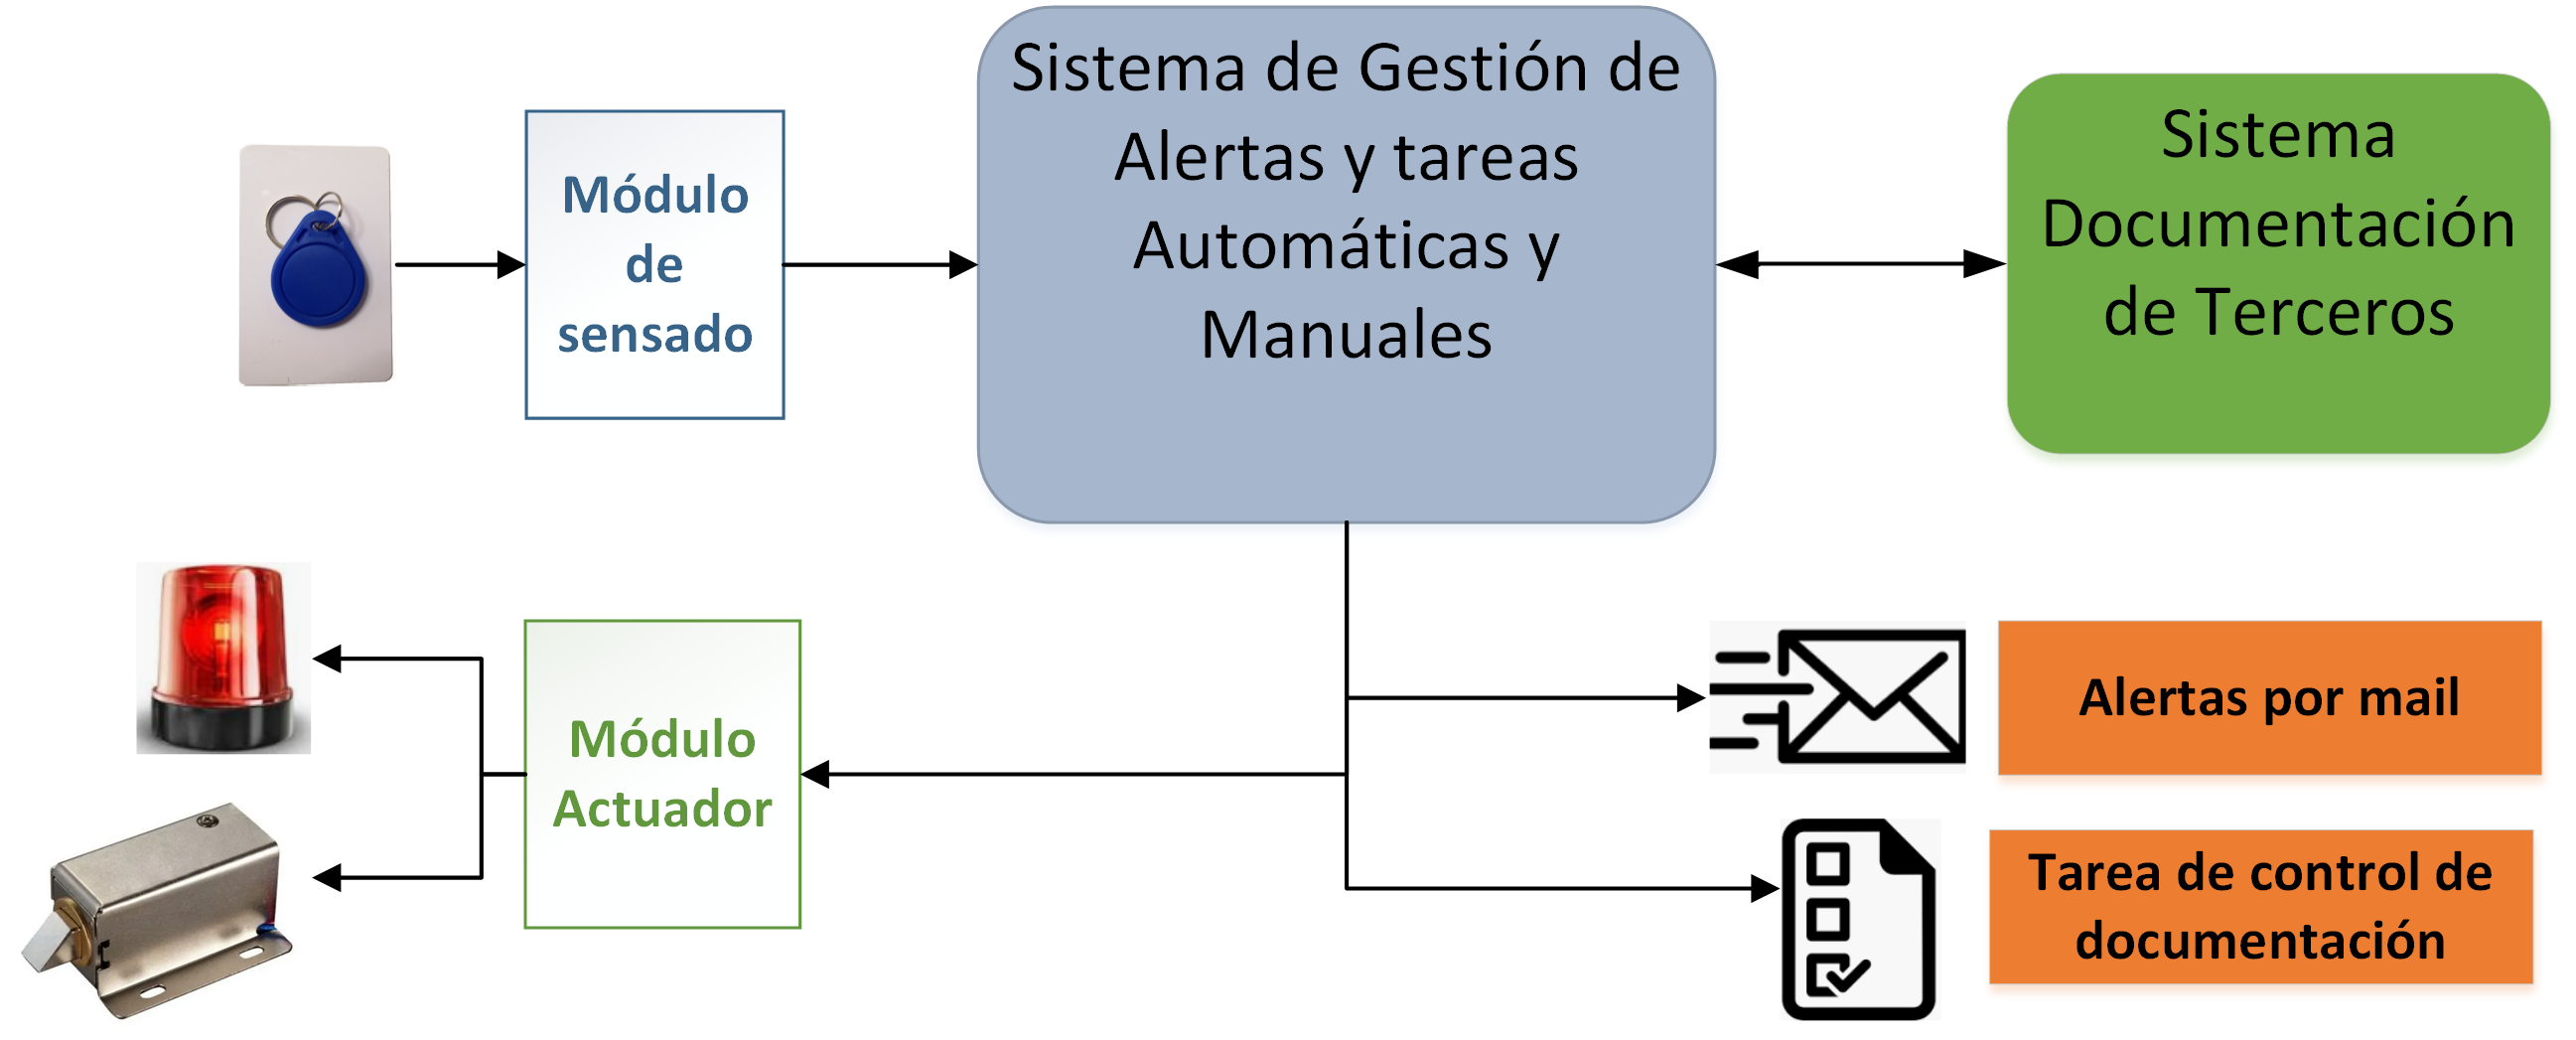
\includegraphics[width=1\textwidth]{./Figures/solucionbasica.png}
	\caption{Diagrama en bloques de la solución propuesta.}
	\label{fig:Solucionbasica}
\end{figure}


%----------------------------------------------------------------------------------------


\chapter{Introducción específica} % Main chapter title

\label{Chapter2}

%----------------------------------------------------------------------------------------
%	SECTION 1
%----------------------------------------------------------------------------------------

Poner párrafo introductorio.

\section{Protocolos de comunicación}

Descripción de los protocolo de comunicación (Wi-Fi/HTTP) utilizados para IoT.

\subsection{Tecnología de comunicación Wi-Fi}

Descripción de tecnología Wi-Fi.

\subsection{Protocolo HTTP}

Descripción de protocolo HTTP.

\section{Componentes de hardware utilizados}

Descripción de los componentes de hardware utilizados: ESP32, lector de tarjetas, cerradura electrónica.

\subsection{Módulo ESP32}

Descripción del módulo.

\subsection{Módulo RFID RC522}

Descripción del módulo.

\subsection{Cerradura electrónica}

Descripción de cerradura.

\section{Tecnologías de software aplicadas}
 
Descripción de las tecnologías de software utilizadas.

\subsection{Node.JS}
\subsection{Ionic}
\subsection{PostgreSQL}
\subsection{MongoDB}
\subsection{Docker}
\subsection{Postman}


\section{Software de control de versiones}

Descripción del software de control de versiones.

\subsection{GitFlow}

Descripción de la herramienta.

\section{Requerimientos}\label{sec:Requerimientos}
 
Requerimientos del proyecto, tanto funcionales, no funcionales, de documentación y de validación. Enumeración de los mismos.
 
\subsection{Requerimientos funcionales}
\begin{enumerate}[label=1.\arabic*]
\item El sistema debe permitir el sensado de datos de distintas fuentes y procesos de planta.
\item El sistema deberá generar alertas a usuarios finales ante problemas detectados del sensado o situaciones límites/problemas potenciales.
\item El sistema deberá generar tareas de corrección y prevención con un circuito de estados que permita trazar el origen del problema y la solución asociada.
\item El sistema debe permitir hacer un seguimiento de la cantidad de alarmas diarias y mensuales generadas.
\item El sistema debe permitir hacer un seguimiento de la cantidad de tareas diarias y mensuales generadas A su vez, se deberá poder ver la cantidad de tareas cerradas, en curso y su antigüedad en días.
\item El sistema debe permitir gestionar usuarios. La gestión de usuarios incluye dar de alta nuevos usuarios, gestionar la recuperación y cambio de clave de los mismos. Dicho usuario se utilizará para acceder y utilizar el sistema.
\end{enumerate}
\subsection{Requerimientos no funcionales}
\begin{enumerate}[label=2.\arabic*]
\item El sistema deberá ser escalable, de forma de poder agregar más módulos actuadores y de sensado para los procesos de planta a futuro.
\item El sistema deberá ser recuperable ante problemas de hardware o software, de forma de asegurar la disponibilidad y no corrupción de la información, cumpliendo con la política de resguardo de datos de la empresa.
\item El sistema deberá poder operarse aún ante cortes puntuales de energía en algunas áreas, esto es, ante corte que no sean generales de toda la planta. Para ello se deberá contar con una política de suministro alternativo de energía para los servidores donde se ejecute el software. 
\end{enumerate}
\subsection{Requerimientos de documentación}
\begin{enumerate}[label=3.\arabic*]
\item Se debe generar una Memoria Técnica con la documentación de ingeniería detallada.
\item Se debe generar un documento de casos de prueba.
\item Se debe generar un documento de la Infraestructura del sistema y de la configuración por ambiente y pasaje entre  ambientes.
\item Se deberá generar la documentación del sistema y del proyecto en el sistema de aprobación y documentación TPA de la empresa.
\end{enumerate}
\subsection{Requerimientos de validación}
\begin{enumerate}[label=4.\arabic*]
\item Se deberá tener una matriz de trazabilidad entre los casos de uso y los casos de prueba, validando el cumplimiento de cada uno y con la aprobación final del auspiciante.
\end{enumerate}

 
\chapter{Diseño e implementación} % Main chapter title

\label{Chapter3} % Change X to a consecutive number; for referencing this chapter elsewhere, use \ref{ChapterX}

\definecolor{mygreen}{rgb}{0,0.6,0}
\definecolor{mygray}{rgb}{0.5,0.5,0.5}
\definecolor{mymauve}{rgb}{0.58,0,0.82}

%%%%%%%%%%%%%%%%%%%%%%%%%%%%%%%%%%%%%%%%%%%%%%%%%%%%%%%%%%%%%%%%%%%%%%%%%%%%%
% parámetros para configurar el formato del código en los entornos lstlisting
%%%%%%%%%%%%%%%%%%%%%%%%%%%%%%%%%%%%%%%%%%%%%%%%%%%%%%%%%%%%%%%%%%%%%%%%%%%%%
\lstset{ %
  backgroundcolor=\color{white},   % choose the background color; you must add \usepackage{color} or \usepackage{xcolor}
  basicstyle=\footnotesize,        % the size of the fonts that are used for the code
  breakatwhitespace=false,         % sets if automatic breaks should only happen at whitespace
  breaklines=true,                 % sets automatic line breaking
  captionpos=b,                    % sets the caption-position to bottom
  commentstyle=\color{mygreen},    % comment style
  deletekeywords={...},            % if you want to delete keywords from the given language
  %escapeinside={\%*}{*)},          % if you want to add LaTeX within your code
  %extendedchars=true,              % lets you use non-ASCII characters; for 8-bits encodings only, does not work with UTF-8
  %frame=single,	                % adds a frame around the code
  keepspaces=true,                 % keeps spaces in text, useful for keeping indentation of code (possibly needs columns=flexible)
  keywordstyle=\color{blue},       % keyword style
  language=[ANSI]C,                % the language of the code
  %otherkeywords={*,...},           % if you want to add more keywords to the set
  numbers=left,                    % where to put the line-numbers; possible values are (none, left, right)
  numbersep=5pt,                   % how far the line-numbers are from the code
  numberstyle=\tiny\color{mygray}, % the style that is used for the line-numbers
  rulecolor=\color{black},         % if not set, the frame-color may be changed on line-breaks within not-black text (e.g. comments (green here))
  showspaces=false,                % show spaces everywhere adding particular underscores; it overrides 'showstringspaces'
  showstringspaces=false,          % underline spaces within strings only
  showtabs=false,                  % show tabs within strings adding particular underscores
  stepnumber=1,                    % the step between two line-numbers. If it's 1, each line will be numbered
  stringstyle=\color{mymauve},     % string literal style
  tabsize=2,	                   % sets default tabsize to 2 spaces
  title=\lstname,                  % show the filename of files included with \lstinputlisting; also try caption instead of title
  morecomment=[s]{/*}{*/}
}

En el presente capítulo se describe la arquitectura del sistema, el diseño y la implementación del hardware y del software y las herramientas de desarrollo utilizadas. 


%----------------------------------------------------------------------------------------
%	SECTION 1
%----------------------------------------------------------------------------------------
\section{Arquitectura del sistema}

En esta sección se explica la arquitectura propuesta, junto a los módulos implementados y los protocolos de comunicación utilizados para la conexión de los mismos. También se expone como se piensa lograr la escalabilidad del sistema.

En la figura \ref{fig:tp-final-infra} se muestra el diagrama en bloques del sistema, junto a los módulos, las tecnologías utilizadas y los protocolos de comunicación que los conectan.

\vspace{0.7cm}
\begin{figure}[ht]
	\centering
	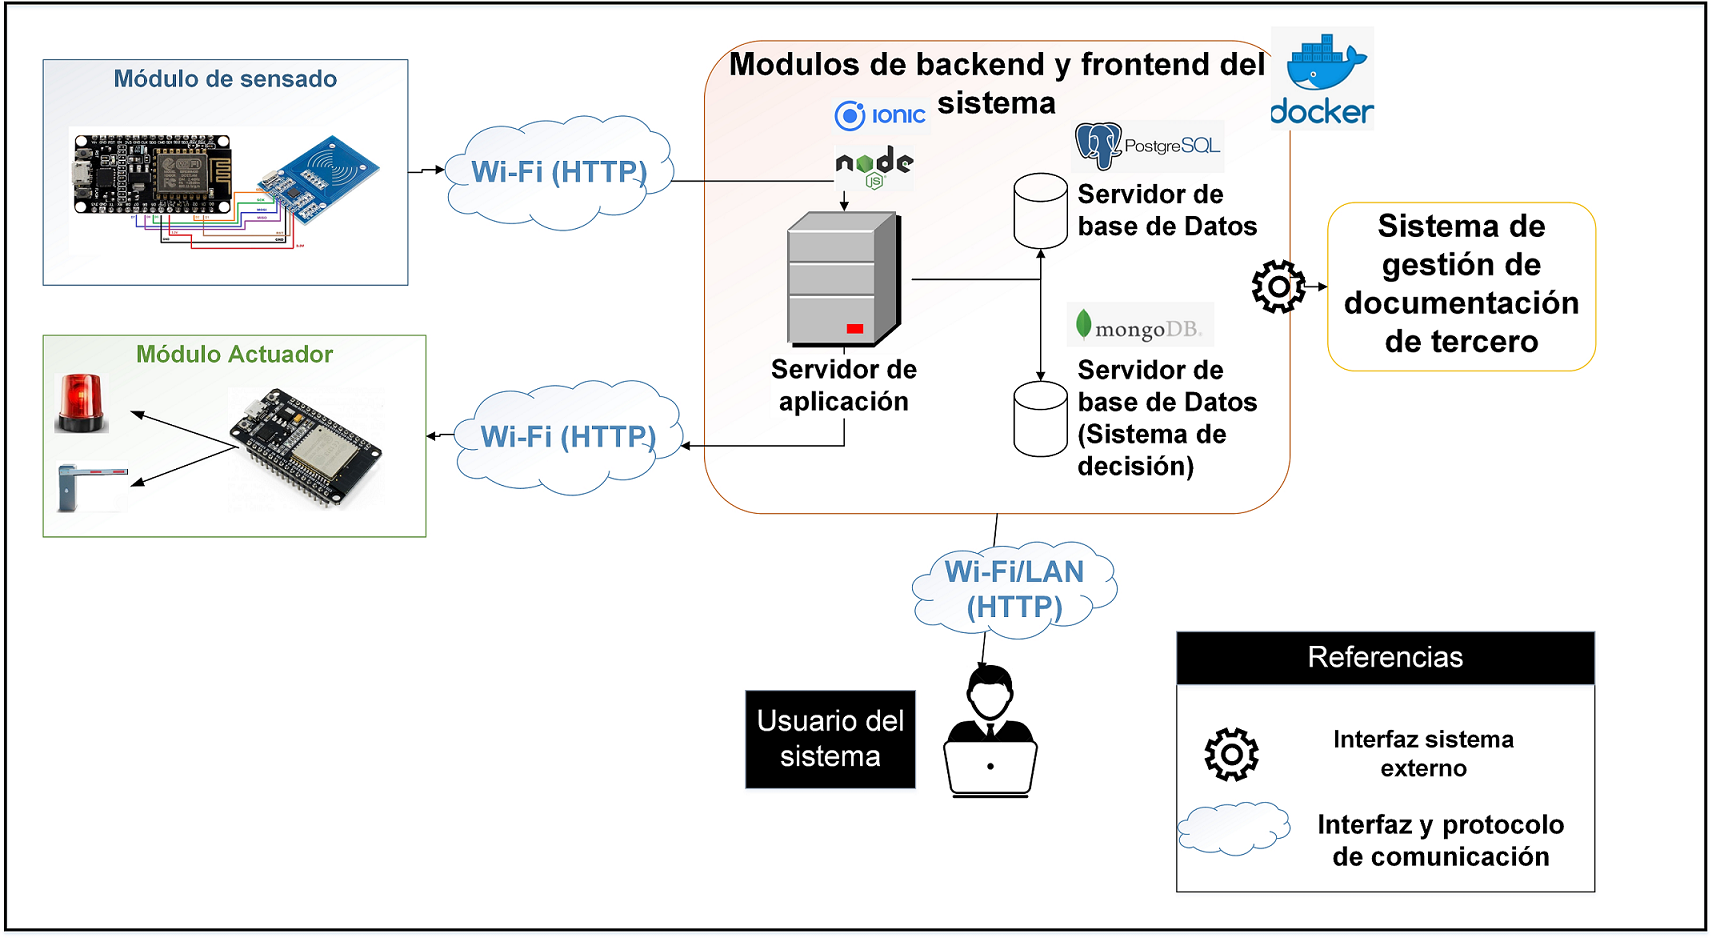
\includegraphics[width=1\textwidth]{./Figures/tp-final-infra.png}
	\caption{Diagrama en bloques del sistema implementado.}
	\label{fig:tp-final-infra}
\end{figure}

\pagebreak
\subsection{Módulos del sistema}

El trabajo desarrollado se divide en los siguientes módulos:

\begin{itemize}
\item Módulo de sensado: es el encargado de leer la tarjeta RFID del personal de tercero que quiere ingresar a la planta y enviar la información al módulo de backend para analizar si la persona cumple con los requisitos para acceder o no.
\item Módulo actuador: es el encargado de comandar la cerradura electrónica que permite o evita el ingreso del tercero a la locación industrial. El mismo recibe las órdenes de cómo operar desde el módulo de backend.
\item Módulos de backend y frontend: si bien estos módulos están implementados de manera conjunta en un único servidor de aplicación, cumplen funciones diferentes:

	\begin{itemize}
	\item Módulo de frontend: es el encargado de brindar una interfaz gráfica a los usuarios, para que estos puedan interactuar con la aplicación, recibiendo sus solicitudes y proporcionándoles la información en un formato simple.
	\item Módulo de backend: es quien gestiona todas las solicitudes provenientes del módulo de sensado y del módulo de frontend. Es el encargado de analizar las solicitudes y responder a las mismas. Cuando recibe peticiones del frontend responde al mismo. Cuando recibe peticiones del módulo de sensado, actúa enviándole órdenes o comandos al módulo actuador. También es el encargado de comunicarse con el sistema de gestión de documentación de terceros. Para cumplir con sus funciones utiliza información almacenada en los servidores de base de datos.
	\end{itemize}
\item Sistema de gestión de documentación de terceros: este sistema es externo y no fue parte del desarrollo. El módulo de backend utiliza el mismo para obtener información de los terceros y en base a ésta tomar las decisiones de habilitar o inhabilitar el acceso y generar alertas y tareas de control.
\end{itemize}

\subsection{Protocolos de comunicación entre módulos}
Para la comunicación entre los módulos se utilizaron invocaciones HTTP GET y POST. 
Tomando como referencia el modelo TPC/IP \citep{WEBSITE:modeloTCPIP}, en la tabla \ref{tab:protocolosComunicacionCap3} se muestra el detalle de protocolos empleados en cada capa:


\begin{table}[h]
	\centering
	\caption[Protocolos comunicación]{Protocolos de comunicación empleados por el sistema.}
	\begin{tabular}{p{3.5cm} p{8.5cm} } 	

		\toprule
		\textbf{Capa del modelo} & 
		\textbf{Protocolo}
		\\
		\midrule

Aplicación & HTTP (utilizando los verbos GET y POST)\\ 
Transporte & TCP\\
Internet & IP (IPv4)\\
Acceso al medio & Wi-Fi (802.11n) para la comunicación entre módulos.

Wi-Fi o IEEE 802.3 (Ethernet) para la comunicación entre el usuario y el módulo de frontend.\\
		\bottomrule
		\hline
	\end{tabular}
	\label{tab:protocolosComunicacionCap3}
\end{table}

Para la elección de los protocolos, se tomó en cuenta las tecnologías disponibles en la empresa. Además, al utilizar protocolos abiertos, estándares y extendidos mundialmente, se logró un sistema portable y adaptable.

\subsection{Tecnologías de bases de datos}

El sistema en general y el módulo de backend en particular, se soporta en dos bases de datos:

\begin{itemize}
\item Una base de datos relacional, implementada en PostgreSQL, que es la que contiene todos los objetos necesarios para la aplicación: usuarios, sensores, actuadores, terceros, eventos del sistema, tareas y sub-tareas de control. 
\item Una base de datos no relacional, implementada en MongoDB, que es utilizada por el backend para almacenar la relación entre los eventos de entrada y el conjunto de acciones que se deben tomar en función de dichos eventos. La decisión de utilizar una base no relacional se debe a que cada tipo de evento de entrada genera diferentes tipos de acciones de salida. Por ejemplo, en el caso de un evento de ingreso de un tercero con documentación en regla solo se debe realizar una acción de apertura de cerradura para el módulo actuador. Pero para un evento de ingreso con documentación vencida se deben generar acciones para cerrar la cerradura en el módulo actuador, generar tareas de control para diferentes sectores de planta y enviar un mail a las personas definidas por la gerencia de la empresa. 

\end{itemize}

\subsection{Contenedores docker y escalamiento}

A fin de generar una solución escalable y modular, se utilizaron contenedores docker para implementar el módulo de backend, el módulo de frontend y para levantar las instancias de base de datos, tanto PostgreSQL como MongoDB. Esta decisión permitió:

\begin{itemize}
\item Simplificar el \textit{deploy} de la aplicación: facilitando la configuración del servidor o servidores donde se ejecuta el sistema.
\item Lograr la escalabilidad futura de la solución: al permitir utilizar un orquestador de contenedores como Kubernetes que permite crear o eliminar instancias de cada contenedor dinámicamente en función de diferentes variables, como el consumo de recursos o la cantidad de solicitudes por segundo. Una ventaja adicional es que, si migramos la solución a la nube, al utilizar este esquema de contenedores dinámicos podemos reducir el costo del servicio, dado que estaremos pagando solo por los contenedores que necesitamos en cada instante de tiempo, sin necesidad de tener un número fijo de recursos en todo momento.
\end{itemize}

\pagebreak
\section{Detalle de módulos de hardware}

En esta sección se describe detalladamente la implementación de los dos módulos de hardware desarrollados en el proyecto. El módulo sensor, encargado de la lectura de las tarjetas RFID del personal de tercero, y el módulo actuador, encargado de gestionar la cerradura electrónica para permitir o evitar el ingreso de dicho personal.

\subsection{Módulo sensor}

Es el encargado de leer las tarjetas RFID del tercero y enviar el valor que tiene la misma al módulo de backend.

Cada tarjeta RFID tiene un valor numérico guardado de 4 caracteres de longitud. Las tarjetas permiten definir valores de hasta 16 caracteres, pero dado que la empresa utiliza códigos de 4 caracteres se colocó ese límite para tener uniformidad.

El módulo está compuesto por los siguientes componentes:

\begin{itemize}
\item Un lector de tarjetas RFID RC522. La elección del mismo se debió a su bajo costo, alta disponibilidad en el mercado y su capacidad para leer las tarjetas que tiene la empresa, que operan en la frecuencia de 13,56 MHz.
\item Un \textit{SoC} (System on a chip) ESP32-WRROM-32. La elección del mismo se debió a su bajo costo, alta disponibilidad en el mercado, facilidad de programación y soporte de redes Wi-Fi (normas 802.11 b/g/n). Esto último simplifica la comunicación del módulo con el backend y evita tener que conectarse a la red LAN de la empresa, lo que hubiera requerido hacer una extensión del cableado de la misma.
\item Un conjunto de leds, que permite al usuario conocer el estado del sistema y el estado de sus interacciones con el módulo. Para ello se dispuso un grupo de 3 leds generales de control y otro de 3 leds de respuesta ante las comunicaciones con el backend.

\end{itemize}

En la figura \ref{fig:moduloSensor} se muestra el módulo sensor junto a sus componentes.

\begin{figure}[ht]
	\centering
	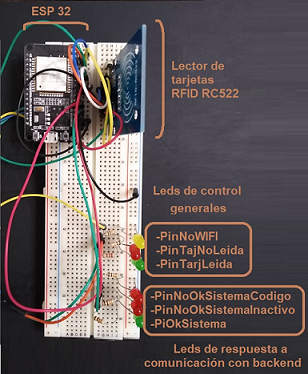
\includegraphics[width=1\textwidth]{./Figures/moduloSensor.png}
	\caption{Módulo sensor junto a sus componentes.}
	\label{fig:moduloSensor}
\end{figure}

\subsubsection{Configuraciones y variables del módulo}

Para implementar este módulo, se desarrolló un programa en el entorno Arduino IDE. El mismo lee las tarjetas RFID y se comunica con el backend, enviando los datos requeridos para procesar el intento de ingreso. Dicha comunicación se realiza a través de la red Wi-Fi de la empresa.

\pagebreak
El módulo cuenta con un conjunto de variables a configurar para su correcta operación:

\begin{itemize}
\item WIFI\_SSID: especifica el SSID de la red Wi-Fi de la empresa.
\item WIFI\_PASSWORD: especifica el password de la red Wi-Fi de la empresa.
\item ID\_SENSOR: especifica el ID que tiene el sensor en la base de datos del sistema. Los datos de cada sensor se almacenan en dicha base de datos, la cual incluye su estado, descripción, ubicación y token asociado.
\item tokenlocal: especifica el token de 20 caracteres que tiene asociado el sensor en la base de datos. Con este valor se asegura la autenticación del módulo.
\item servicioAPISensor: contiene la URL del endpoint que expone el backend para recibir los datos de este módulo.
\end{itemize}

\subsubsection{Comunicación con el backend}

El módulo tiene configurada la dirección URL del endpoint que el backend expone para permitir la comunicación entre éstos.

Para enviar los datos solicitados, se realiza un HTTP POST con un objeto JSON que tiene 3 claves:

\begin{itemize}
\item id: contiene el valor ``ID\_SENSOR'' del módulo.
\item token: contiene el valor de ``tokenlocal'' del módulo.
\item valor: contiene el valor leído de la tarjeta RFID, que representa al id del tercero en el sistema.
\end{itemize}

Una vez enviado el HTTP POST, el módulo recibe como respuesta un valor que indica si los datos mandados son correctos o si hubo algún error. Con esta respuesta se determina qué leds deben activarse para dar \textit{feedback} al usuario del estado del proceso.

\subsubsection{Leds del sistema}

El módulo cuenta con un conjunto de leds, que permiten al usuario conocer el estado del mismo y el resultado de sus interacciones con éste.

Cuando el mismo se inicializa hace un chequeo de estos leds, prendiéndolos y apagándolos, uno a uno, durante medio segundo.

En la tabla \ref{tab:combinacionLedsSensor} se muestra el detalle de los leds o combinaciones posibles de leds, junto a la información que brindan al usuario cuando se encienden.

\begin{table}[h]
	\centering
	\caption[Leds módulo sensor ]{Combinación de leds e información para el usuario cuando se prenden.}
	\begin{tabular}{p{4cm} p{8.5cm} } 	

		\toprule
		\textbf{Led/combinación de leds} & 
		\textbf{Información para el usuario}
		\\
		\midrule

PinNoWIFI & Al leer la tarjeta del tercero, si no se cuenta con comunicación Wi-Fi con el backend, el led se prende durante 3 segundos.\\ 
PinTarjNoLeida & Falló la lectura de la tarjeta o la misma no tiene valor asignado. Se debe configurar la tarjeta con el valor correspondiente al personal de tercero.\\
PinTarjLeida & Al acercar la tarjeta al lector, el sistema lee correctamente la misma, junto al valor que tiene almacenado.\\
PinOkSistema & Una vez leída la tarjeta del personal de tercero, el sistema se comunica correctamente con el backend. Se informa al usuario al prender el led durante 2 segundos. \\
PinNoOkSistemaCodigo & Una vez leída la tarjeta del personal de tercero, el sistema se comunica correctamente con el backend, pero el valor de ``ID\_SENSOR'' enviado no se corresponde con ningún módulo sensor configurado en el sistema, o el mismo está inactivo. Se informa al usuario al prender el led durante 2 segundos. \\
PinNoOkSistemaCodigo
+
PinNoOkSistemaInactivo & Una vez leída la tarjeta del personal de tercero, el sistema se comunica correctamente con el backend, pero éste devuelve un error con un código no especificado. Se informa al usuario al prender el ``led PinNoOkSistemaCodigo'' durante 1 segundo seguido del led ``PinNoOkSistemaInactivo'' durante otro segundo.
\\
		\bottomrule
		\hline
	\end{tabular}
	\label{tab:combinacionLedsSensor}
\end{table}


\subsection{Módulo actuador}

Es el encargado de comandar la cerradura. El mismo cuenta con un conjunto de leds que brindan información al personal de tercero del estado del módulo y del estado de su ingreso.

Las órdenes de cómo operar las recibe desde el módulo de backend, para lo cual el actuador expone un \textit{endpoint} HTTP, que recibe un JSON con dichas órdenes.

\pagebreak
El módulo está compuesto por los siguientes componentes:

\begin{itemize}
\item Un \textit{SoC} ESP32-WRROM-32. La elección del mismo se debió a su bajo costo, alta disponibilidad en el mercado, facilidad de programación y soporte de redes Wi-Fi (normas 802.11 b/g/n). Esto último simplifica la comunicación del módulo con el backend y evita tener que conectarse a la red LAN de la empresa, lo que hubiera requerido hacer una extensión del cableado de la misma.
\item Un regulador de tensión, que brinda los niveles de tensión requeridos para energizar el ESP32 y para la activación del Mosfet IRF520. 
\item Cerradura electrónica. La misma se acciona y alimenta desde el Mosfet IRF520.
\item Conversor de niveles lógicos. Se utiliza para convertir la tensión de salida del ESP32 (3.3 V) a la tensión requerida para accionar el Mosfet IFR520 (5V).
\item Mosfet IRF520: permite accionar la cerradura electrónica, brindando el nivel de tensión requerida por la misma (12 V).
\item Un conjunto de leds, que permiten conocer si el actuador está encendido y el estado del ingreso del tercero (habilitado/inhabilitado/error).
\item Fuente de alimentación de 12 V, que es utilizada para alimentar el  Mosfet IRF520 y al regulador de tensión.
\end{itemize}

En la figura \ref{fig:moduloActuador} se muestra el módulo actuador con sus componentes.

\begin{figure}[ht]
	\centering
	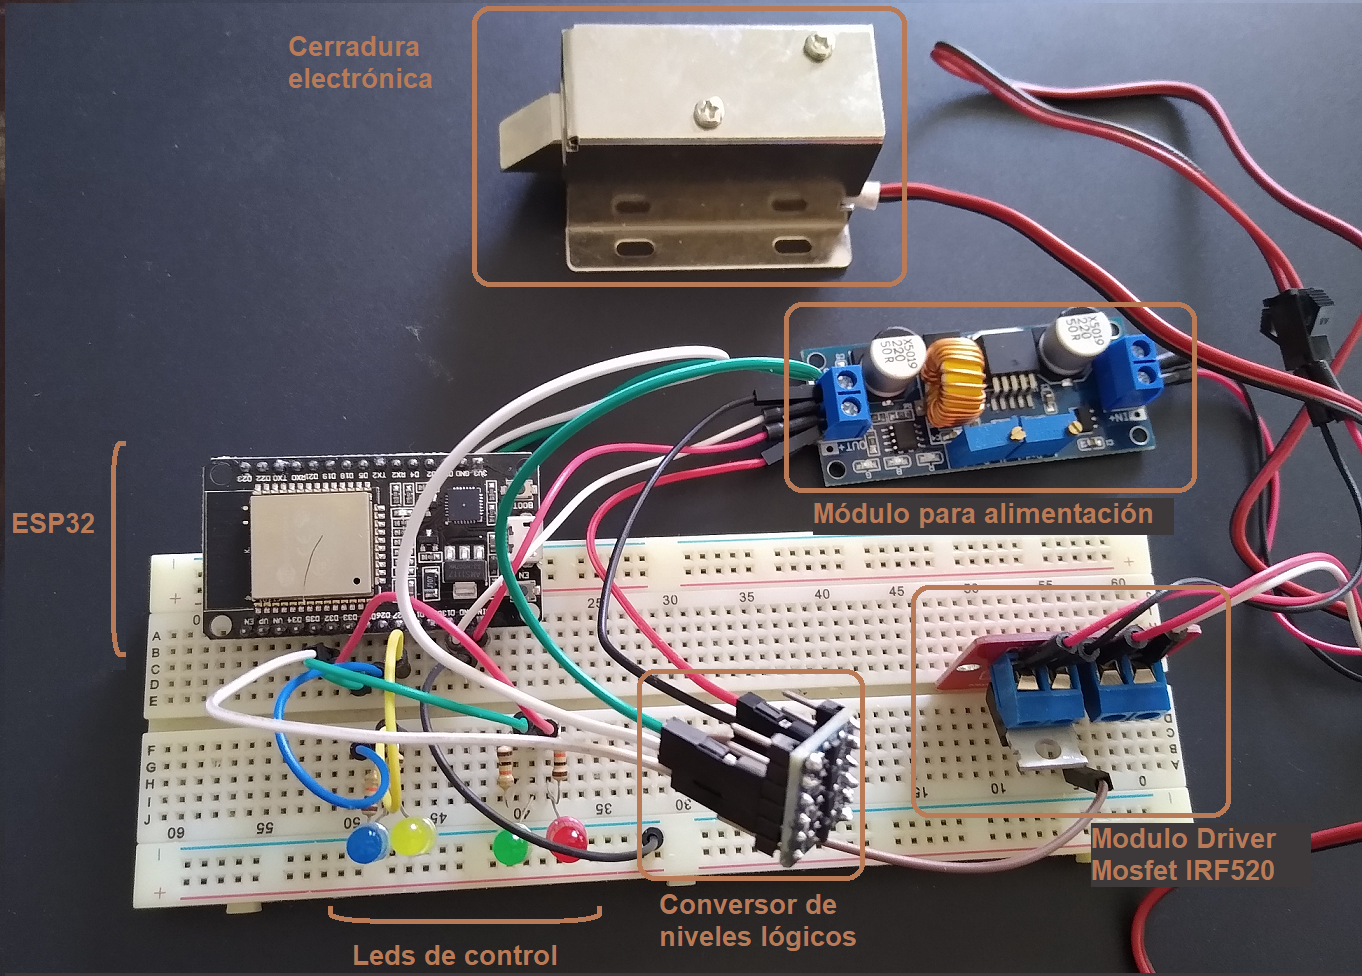
\includegraphics[width=1\textwidth]{./Figures/moduloActuador.png}
	\caption{Módulo actuador junto a sus componentes.}
	\label{fig:moduloActuador}
\end{figure}

\subsubsection{Configuraciones y variables del módulo}

Para implementar el actuador, se desarrolló un programa en el entorno Arduino IDE. Este programa expone un \textit{endpoint} HTTP POST, que recibe un JSON con las acciones a realizar. En función de la acción y valor indicados, se acciona la cerradura electrónica y se prenden los leds de control.

En la base de datos del sistema se guarda la información de los actuadores existentes, su ubicación, descripción, estado, dirección IP y token de autenticación.

El actuador cuenta con un conjunto de variables a configurar para su correcta operación:

\begin{itemize}
\item WIFI\_SSID: especifica el SSID de la red Wi-Fi de la empresa.
\item WIFI\_PASSWORD: especifica el password de la red Wi-Fi de la empresa.
\item tokenlocal: especifica el token de 20 caracteres que tiene asociado el actuador en la base de datos. Con este valor se asegura la autenticación del módulo.
\item local\_IP: especifica la dirección IP del mismo. Se utiliza una IP fija, para asegurar que el \textit{endpoint} expuesto siempre pueda ser accedido. Si se utilizara una IP dinámica la dirección podría cambiar y quedaría inaccesible dicho \textit{endpoint}.
\item Subnet: dirección de sub-red de la red Wi-Fi.
\end{itemize}

\subsubsection{Comunicación desde el backend}

El módulo recibe un HTTP POST desde el backend con un objeto JSON que tiene 3 claves:

\begin{itemize}
\item token: contiene el token de autenticación.
\item acción: contiene la acción a realizar. Es un clasificador de acciones posibles.
\item valor: contiene el valor particular para la acción.
\end{itemize}

Al recibir el objeto se controla si el token coincide con el valor de token que se tiene almacenado localmente, y luego se controla si la acción y valor son válidos. En función de la acción y valor, se abre o cierra la cerradura, y prende el led de ingreso ok, de ingreso no ok o de error. Por último, se responde al backend con un código de error o un ok.

\subsubsection{Detalle de respuestas ante solicitudes del backend}

El backend realiza solicitudes al actuador como se explica en la sub-sección anterior. En la tabla \ref{tab:respuestasActuadorBackend} se muestra el detalle las diferentes combinaciones de valores que puede recibir el módulo en las solicitudes y se indica la respuesta brindada al usuario y al backend.


\begin{table}[h]
	\centering
	\caption[Respuestas backend ]{Respuestas posibles del módulo al usuario y al backend ante las solicitudes recibidas.}
	\begin{tabular}{p{4cm} p{4.5cm} p{4.5cm} } 	

		\toprule
		\textbf{Valores recibidos} & 
		\textbf{Respuesta al usuario} &
		\textbf{Respuesta al backend} 
		\\
		\midrule

Acción=``APERTURA''

Valor=``ABRIR''

Token con valor correcto.& Se prende el led verde de manera intermitente durante 4 segundos. Durante ese tiempo la cerradura electrónica se cierra. & Se envía respuesta HTTP con código 200 y mensaje OK. \\
Acción=``APERTURA''

Valor=``CERRAR''

Token con valor correcto. & Se prende el led rojo durante 2 segundos. & Se envía respuesta HTTP con código 200 y mensaje ``Sin token de autenticación.'' \\
Sin token. & Se prende el led amarillo  durante medio segundo y se apaga. & Se envía respuesta HTTP con código 401 y mensaje ``Sin token de autenticación.'' \\
Token con valor incorrecto. & Se prende el led amarillo  durante medio segundo y se apaga. & Se envía respuesta HTTP con código 403 y mensaje ``Token de autenticación incorrecto.'' \\
Acción no especificada o con valor incorrecto. & Se prende el led amarillo de manera intermitente durante 2 segundos. & Se envía respuesta HTTP con código 400 y mensaje ``La acción especificada no es válida.'' \\
Valor no especificado o valor incorrecto. & Se prende el led amarillo de manera intermitente durante 3 segundos. & Se envía respuesta HTTP con código 400 y mensaje ``El valor especificado no es válido''. \\
		\bottomrule
		\hline
	\end{tabular}
	\label{tab:respuestasActuadorBackend}
\end{table}

\pagebreak
\section{Detalle de módulos de software}

En esta sección se describe detalladamente la implementación de los dos módulos de software desarrollados en el proyecto: el de backend, encargado tanto de recibir las solicitudes del módulo sensor y de frontend como de enviar comandos al actuador, y el módulo de frontend, encargado de gestionar las solicitudes del usuario mediante una interfaz gráfica.

\subsection{Módulo de backend}

El mismo está implementado como una aplicación web con Node.JS, utiliza las librerías Express y Socket.io y expone:

\begin{itemize}
\item Una API Rest para el frontend, la cual responde a sus solicitudes e incluye un WebSocket para mostrar alertas online a la Portería.
\item Una API de autenticación, utilizada para la gestión e inicio de sesión de los usuarios.
\item Un \textit{endpoint} para recibir las solicitudes de ingreso del módulo sensor.
\end{itemize}

Para su desarrollo se utilizó el IDE Visual Studio Code. Dentro del mismo se organizaron las carpetas con el código y las configuraciones para el testing automático.

En la figura \ref{fig:backendCarpetas}  se muestra la estructura en carpetas definidas para el backend.

\begin{figure}[ht]
	\centering
	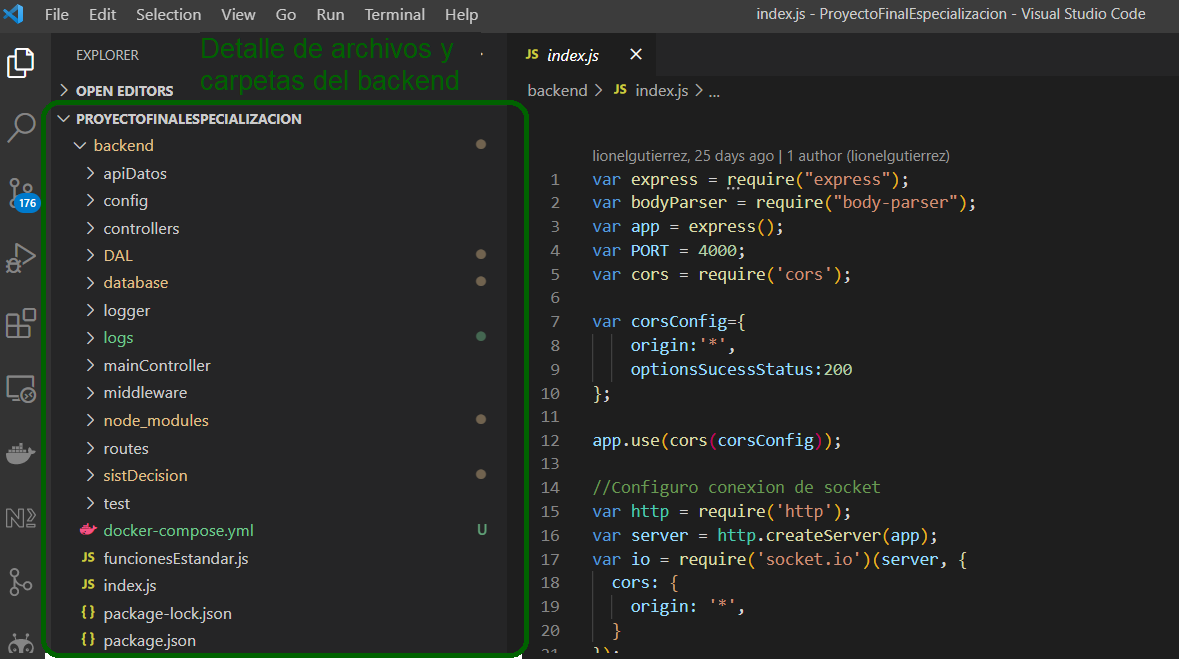
\includegraphics[width=1\textwidth]{./Figures/backendCarpetas.png}
	\caption{Estructura de directorio del backend desarrollado en Visual Studio Code.}
	\label{fig:backendCarpetas}
\end{figure}

En la tabla \ref{tab:carpetasBackend}  se expone detalladamente el contenido y función de cada una de las carpetas y archivos del módulo.

\begin{table}[h]
	\centering
	\caption[Carpetas backend ]{Detalle de archivos y carpetas del módulo de backend.}
	\begin{tabular}{p{2cm} p{11cm}} 	
		\toprule
		\textbf{Archivo/
		Directorio} & 
		\textbf{Descripción} 
		\\
		\midrule
apiDatos & Contiene cada uno de los \textit{endpoints} expuestos al frontend. Se implementó utilizando Express, junto a métodos GET y POST, para servir las consultas de información y las altas y actualizaciones en la base de datos. \\
config & Contiene tanto la configuración del \textit{secret} necesaria para el sub-módulo de autenticación, como la configuración de constantes utilizadas en la comunicación con el sistema de documentación de terceros. \\
controllers & Cuenta con tres controladores:
\begin{itemize}
\item generacionAlertas: es el encargado de comunicarse con el módulo actuador y enviarle los comandos para habilitar o prohibir la solicitud de ingreso del tercero a la planta.
\item generacionMensajes: es el encargado de gestionar el envío de emails a los usuarios requeridos.
\item generacionTareas: es el encargado de generar las tareas y sub-tareas, guardando la información en la base de datos.
\end{itemize} \\
DAL & La DAL (Data Access Layer), es la encargada de abstraer la comunicación con la base de datos, al brindar un conjunto de métodos para acceder y realizar las altas, bajas y modificaciones, sin necesidad de que los componentes que la usan conozcan la implementación subyacente. \\
database & Contiene las configuraciones necesarias para conectarse a la base de datos PostgreSQL. Se utiliza un \textit{pool} de conexiones a fin de mejorar el rendimiento y la escalabilidad del sistema. \\
logger & Es el encargado de gestionar el \textit{logging} de eventos.\\
logs & Almacena los \textit{logs} del sistema. Se guarda un archivo de \textit{log} por día para evitar archivos muy extensos y simplificar la búsqueda de información en los mismos. \\
main

Controller & Es el encargado de gestionar las solicitudes de ingreso del módulo sensor. Se comunica con el sistema de documentación de terceros, determina los tipos de acción a realizar y dispara cada una de ellas, invocando a los controladores de la carpeta controllers.  \\
middleware & Contiene los métodos necesarios para la gestión de la autenticación \\
routes & Contiene cada uno de los \textit{endpoints} expuestos tanto para la API de autenticación (sub-carpeta ``routerAuth'') como para la recepción de datos desde el módulo sensor (sub-carpeta ``routerSensores''). \\
sistDecision & Contiene el sub-módulo que se encarga de determinar las acciones a realizar cuando hay una solicitud de ingreso de un tercero, para lo cual utiliza la base de datos implementada en MongoDB. \\
test & Contiene los archivos necesarios para la ejecución de las pruebas automáticos implementados para la solución. En el capítulo \ref{Chapter4} se explican con mayor detalle las pruebas implementadas y los archivos utilizados. \\
index.js & Contiene la configuración para levantar la aplicación y cada una de las rutas utilizadas por la aplicación. También incluye la configuración de CORS y del WebSocket. \\
		\bottomrule
		\hline
	\end{tabular}
	\label{tab:carpetasBackend}
\end{table}

\clearpage
\subsubsection{API de autenticación}

La API de autenticación se utiliza para segurizar las invocaciones realizadas al backend. Para hacerlo emplea tokens JWT. Además, permite el alta de nuevos usuarios, gestionar el inicio de sesión de los mismos y el cambio y reseteo de passwords.

Para el desarrollo de esta API utilizamos 2 librerías disponibles en node.JS: bcryptjs y jsonwebtoken. La primera permite implementar una función de \textit{hash}, que posibilita guardar encriptado el password de los usuarios. La segunda permite generar el token JWT que es entregado al usuario para que pueda acceder a los diferentes \textit{endpoints}, asegurando su autenticidad. Dicho token tiene una duración de 24 horas.

\subsubsection{Funcionamiento del módulo ante una solicitud del módulo sensor}{\label{sec:subSeccionSolitiudModuloSensor}}   

Cuando el módulo sensor hace una solicitud al backend invoca al \textit{endpoint} de recepción de sensores. El backend, por su parte, recibe la solicitud y realiza los pasos descriptos a continuación: 

\begin{enumerate}
\item Envía el pedido al router ``routerSensores''. 
\item ``routerSensores'' controla el token y valores recibidos. Si el token no es válido o el id de sensor enviado no es correcto o está inactivo, se envía un mensaje de error al origen y se termina la solicitud.
\item Si los datos son correctos, se envían al ``mainController''.
\item El ``mainController'' realiza estas acciones:
	\begin{enumerate}
	\item Se comunica con el sistema de documentación de terceros para determinar si la persona está en condiciones de ingresar. 
	\item Registra el evento de ingreso en la base de datos (no directamente, sino a través de la ``DAL'').
	\item Con los datos obtenidos se comunica con el sub-módulo de decisión (``sistDecision''), el cual le indica las acciones a realizar. 
	\item Para cada una de las acciones indicadas, en función del tipo que sea (de salida, mensaje, tarea), se comunica con los controladores ``generacionAlertas'', ``generacionMensajes'' o ``generacionTareas'', para que éstos las procesen y registren.
	\end{enumerate}
\end{enumerate}

En la figura \ref{fig:DiagramaInteaccion1} se muestra la interrelación entre los componentes del módulo y el flujo de datos ante una solicitud desde el módulo sensor.

\begin{figure}[ht]
	\centering
	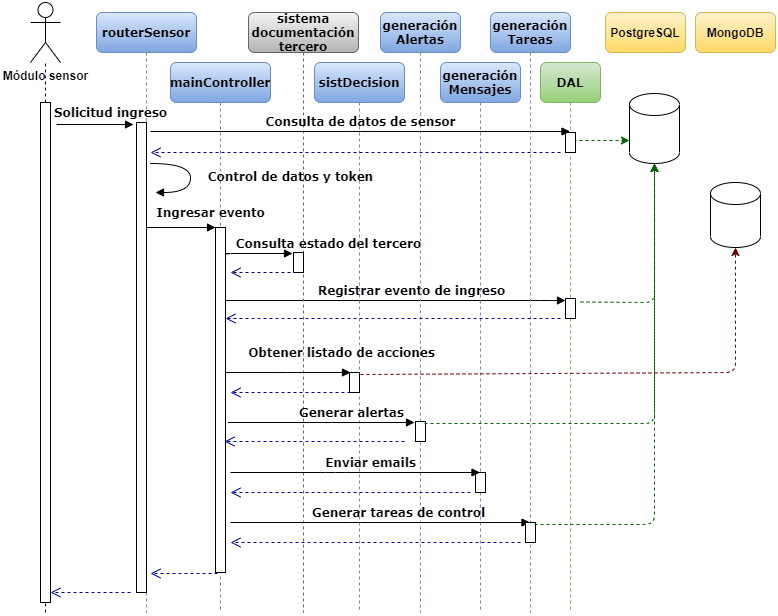
\includegraphics[width=1\textwidth]{./Figures/DiagramaInteaccion1.png}
	\caption{Interacción entre los componentes del módulo ante una solicitud del módulo sensor.}
	\label{fig:DiagramaInteaccion1}
\end{figure}

\pagebreak
\subsubsection{Funcionamiento del módulo ante una solicitud del módulo de frontend}

Cuando el módulo de frontend hace una solicitud al backend invoca algunos de los \textit{endpoints} definidos en ``apiDatos''. El backend, por su parte, recibe la solicitud y realiza los pasos descriptos a continuación: 
\begin{enumerate}
\item Envía el pedido a ``apiDatos''. 
\item ``apiDatos'' determina el endpoint solicitado, pasa el control al mismo y éste realiza las siguientes acciones:
	\begin{enumerate}
	\item Controla que la solicitud tenga el token de autenticación y lo valida utilizando las funciones del \textit{middleware} de autenticación.
	\item Si el token no es correcto se rechaza el pedido con un código 403.
	\item Si el token es correcto, opcionalmente y según la necesidad de cada \textit{endpoint}, controla el rol de usuario asociado al token utilizando nuevamente el \textit{middleware} de autenticación.
	\item Si el rol/roles solicitados no son correctos rechaza el pedido con un código 403.
	\item Si los roles son correctos procede con la solicitud. En general cada solicitud controla los datos de entrada y luego se comunica con la base de datos a través de la ``DAL'', ya sea para consultar, agregar o modificar información.
	\end{enumerate}

\end{enumerate}

En la figura \ref{fig:DiagramaInteraccion2} se muestra la interrelación entre los componentes del módulo y el flujo de datos ante una solicitud desde el frontend.

\begin{figure}[ht]
	\centering
	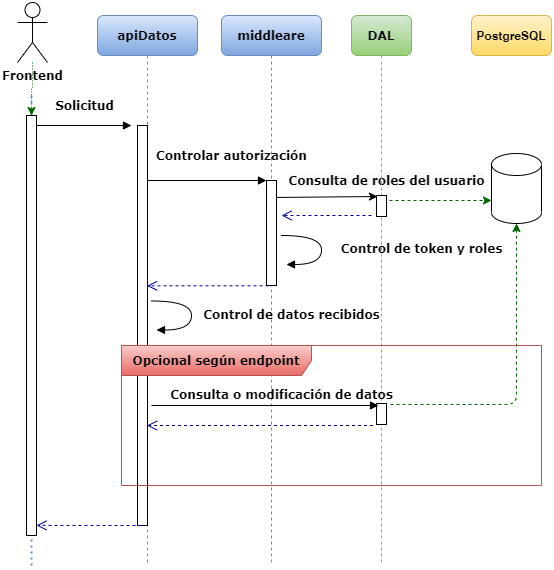
\includegraphics[width=1\textwidth]{./Figures/DiagramaInteraccion2.png}
	\caption{Interacción entre los componentes del módulo ante una solicitud del frontend.}
	\label{fig:DiagramaInteraccion2}
\end{figure}

\subsection{Módulo de frontend}

Este módulo brinda una interfaz gráfica al usuario a través de la cual interactúa con el sistema, ya sea para consultar datos o para registrar acciones. Con el objetivo de cumplir con tales funciones se comunica con el backend a través de una API Rest. Para su desarrollo se empleó Angular y el framework Ionic. Su utilización permitió construir el sistema como una aplicación web responsive con la idea de implementarla a futuro como una \textit{app mobile}. Para la escritura del código fuente apelamos al IDE Visual Studio Code. Dentro del mismo se organizaron las carpetas con el código y cada uno de los diferentes elementos.

\pagebreak
En la figura \ref{fig:frontendCarpetas} se muestra la estructura en carpetas definidas para el frontend.

\begin{figure}[ht]
	\centering
	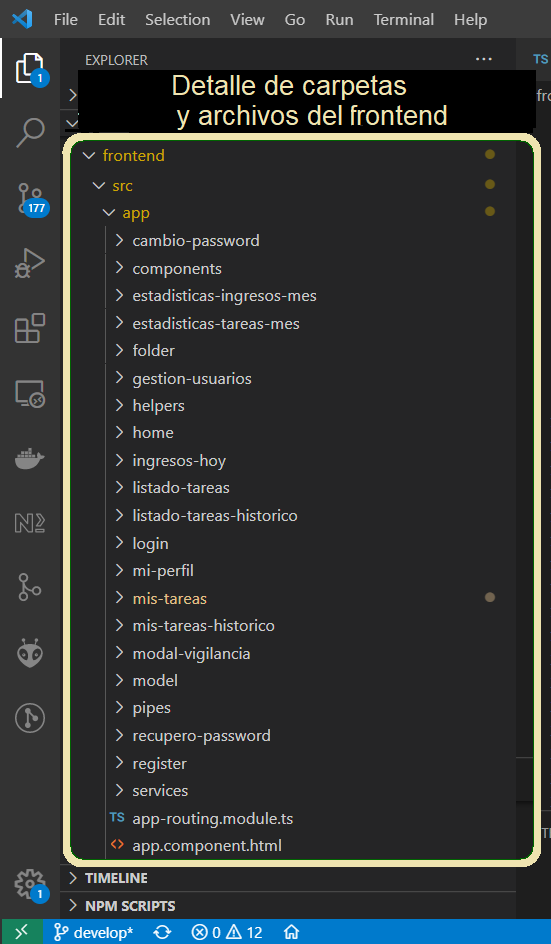
\includegraphics[width=1\textwidth]{./Figures/frontendCarpetas.png}
	\caption{Estructura de directorio del frontend desarrollado en Visual Studio Code.}
	\label{fig:frontendCarpetas}
\end{figure}


En la tabla \ref{tab:carpetasFrontend}  se expone detalladamente el contenido y función de cada una de las carpetas y archivos del módulo.

\begin{table}[h]
	\centering
	\caption[Carpetas frontend ]{Detalle de archivos y carpetas del módulo de frontend.}
	\begin{tabular}{p{2.3cm} p{10.7cm}} 	
		\toprule
		\textbf{Archivo/
		Directorio} & 
		\textbf{Descripción} 
		\\
		\midrule
cambio-password & Contiene la página que gestiona el cambio de password de los usuarios. \\
components & Contiene tres sub-carpetas con los componentes desarrollados para la solución. Los componentes implementados son:
\begin{itemize}
\item estadística-evento-fecha: muestra la cantidad de ingresos habilitados y rechazados en el día.
\item listar-tareas: muestra una grilla con el listado de tareas y sub-tareas en un rango de fechas y con un estado particular. 
\item tareas-usuario: muestra un listado con cada una de las sub-tareas que tiene un usuario.
\end{itemize} \\
estadísticas-ingreso-mes & Contiene la página que muestra las estadísticas de cantidad de ingresos por mes.\\
estadisticas-tareas-mes & Contiene la página que muestra las estadísticas de cantidad de tareas cerradas por año.\\
gestión-usuarios & Contiene la página que muestra el listado de usuarios del sistema y permite cambiar el estado de los mismos (activo/inactivo) y agregarles o quitarles roles. \\
helpers & Contiene la clase ``authInterceptor'' que permite enviar cada solicitud al backend con el token de autenticación. Para esto intercepta el pedido HTTP y le agrega al encabezado dicho token. \\
home & Contiene la página principal de la aplicación que muestra, según el rol del usuario, las estadísticas de ingreso al sistema o las tareas en curso del mismo.\\
ingresos-hoy & Contiene la página que muestra el listado de ingresos del día con la fecha de cada ingreso y si el usuario fue habilitado o no. \\
listado-tareas & Contiene la página que muestra el listado de tareas en curso. Utiliza el componente ``listar-tareas''. \\
listado-tareas
-historico & Contiene la página que muestra el listado de tareas completas. Utiliza el componente ``listar-tareas''. \\
login & Contiene la página de inicio de sesión para los usuarios. \\
mi-perfil & Contiene la página que muestra el perfil de usuario y sus datos. \\
mis-tareas & Contiene la página que muestra las tareas en curso asignadas al usuario. \\
mis-tareas
-historico & Contiene la página que muestra las tareas cerradas del usuario. \\
model & Contiene las clases que representan a los objetos de negocio del sistema: roles, usuarios, tareas, sub-tareas, sectores. \\
pipes & Contiene la implementación de un \textit{pipe}, que define diferentes colores en función del valor de entrada recibido. Sirve para alertar al usuario de la antigüedad de sus tareas. \\
recupero-password & Contiene la página que permite al usuario recuperar su password. \\
register & Contiene la página que permite dar de alta nuevos usuarios al sistema. \\
services & Contiene los servicios que utilizan las diferentes páginas y componentes para gestionar sus datos y consultas al backend. \\
		\bottomrule
		\hline
	\end{tabular}
	\label{tab:carpetasFrontend}
\end{table}

\clearpage
\subsubsection{Detalle de servicios (``services'') implementados}
En esta sub-sección se detallan los servicios implementados en Angular. Mientras que los componentes y las páginas están enfocados en brindar una interfaz gráfica simple y fácil de utilizar para los usuarios, los servicios se orientan a las tareas de lógica de negocio, lo que incluye comunicarse con el backend y gestionar la autenticación y los datos del usuario.

Los servicios implementados son los siguientes:

\begin{itemize}
\item authService: se comunica con la API de autenticación del backend para gestionar los inicios de sesión, el alta de nuevos usuarios y las funcionalidades de recuperación y cambio de password.
\item camibioMenuService: se encarga del armado del menú de aplicaciones del usuario, en función de su rol. 
\item datosAuxiliaresService: se encarga de comunicarse con el backend para consultar los datos auxiliares del sistema que son de acceso público como, por ejemplo, el listado de sectores de planta para la pantalla de alta de nuevos usuarios.
\item ingresosService: se comunica con el backend para obtener la información de ingresos a planta por rango de fechas.
\item socketService: gestiona el socket utilizado para que la vigilancia y la gerencia puedan visualizar en tiempo real los ingresos a la planta.
\item tareaService: se comunica con el backend para obtener información de las tareas en curso, de las tareas cerradas y para realizar modificaciones en las mismas.
\item tokenStorageService: es el encargado de la gestión del token de autenticación que devuelve el backend al iniciar sesión. Dentro de la gestión se incluye su almacenamiento y recuperación.
\item usuariosService: se comunica con el backend para realizar cambios en el estado de los usuarios y sus roles. Solo es utilizado por el rol administrador. 
\item loginGuardService: permite al módulo de ruteo de la aplicación controlar que el usuario cuente con el rol necesario para acceder a una determinada página. Este servicio se utiliza para habilitar los accesos a las páginas solo al rol de usuario normal.
\item rolAdminGuardService: permite al módulo de ruteo de la aplicación controlar que el usuario cuente con el rol necesario para acceder a una determinada página. Este servicio se utiliza para habilitar los accesos a las páginas solo al rol de usuario administrador.
\item rolAGerenteGuardService: permite al módulo de ruteo de la aplicación controlar que el usuario cuente con el rol necesario para acceder a una determinada página. Este servicio se utiliza para habilitar los accesos a las páginas solo al rol de usuario gerente.
\item rolVigilanciaGuardService: permite al módulo de ruteo de la aplicación controlar que el usuario cuente con el rol necesario para acceder a una determinada página. Este servicio se utiliza para habilitar los accesos a las páginas solo al rol de usuario vigilancia.
\end{itemize}

\subsubsection{Funcionamiento del módulo ante un inicio de sesión}

En este apartado se explica el inicio de sesión de un usuario, en el que se puede ver la interacción con el backend y el guardado del token de autenticación para futuras consultas.
El proceso comienza cuando el usuario ingresa al sistema y visualiza la pantalla de inicio de sesión. Coloca su username y password y hace click en el botón “Loguearse”. Ante el click del usuario, el sistema realiza las siguientes interacciones:

\begin{enumerate}
\item El módulo ``loginModule'' invoca al servicio ``authService'' con los datos de username y password.
\item ``authService'' se comunica con el backend mediante un HTTP POST a la API de autenticación y recibe como respuesta el token asociado al usuario y los datos del mismo (username, password, email, sector y roles asociados). El servicio envía los datos recibidos al módulo ``loginModule''.
\item El módulo al recibir el token y los datos del usuario utiliza el servicio ``tokenStorageService'' para almacenar los valores. Luego, invoca al servicio ``cambioMenuService'' que genera el menú de usuario según sus roles. Por último, invoca al módulo ``homeModule'' que muestra la página de inicio al usuario. 
\end{enumerate}

En la figura \ref{fig:inisioSesionInteraccion} se muestra el diagrama de interacción para el inicio de sesión.

\begin{figure}[ht]
	\centering
	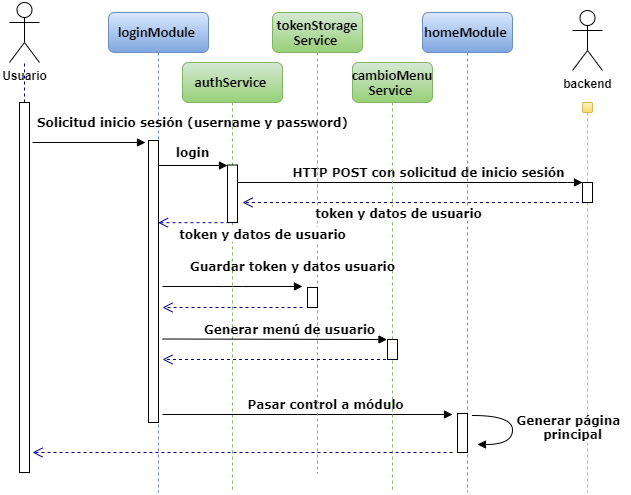
\includegraphics[width=1\textwidth]{./Figures/inisioSesionInteraccion.png}
	\caption{Diagrama de interacción para el inicio de sesión.}
	\label{fig:inisioSesionInteraccion}
\end{figure}

\pagebreak
\subsubsection{Funcionamiento del módulo ante una solicitud de usuario}

En esta sección se explica una interacción típica del usuario en la que se puede ver la relación entre los diferentes elementos del frontend y su comunicación con el backend.

Como pre-requisito, el usuario ya inició sesión en el sistema y desea consultar sus tareas en curso. Para ello hace click en la opción ``Mis Tareas en curso'' del menú de aplicaciones. Ante el click del usuario el sistema realiza las siguientes interacciones:

\begin{enumerate}
\item El módulo de ruteo ``app-routing.module'' determina quién es el encargado de procesar la solicitud del usuario. En nuestro caso es ``mis-tareas-module''. Luego, controla que éste pueda acceder a la página. Para ello consulta con el ``loginGuardService''.
\item Si se determina que se puede acceder a la página, se transfiere el control al módulo ``mis-tareas-module''. Éste invoca al servicio ``tokenStorageService'' para adquirir el token de usuario y su id. Con dicho id llama al servicio ``tareasService'' para obtener las tareas del usuario.
\item El servicio ``tareaService'' genera la solicitud HTTP GET y la envía al backend.
\item El ``authInterceptor'' intercepta la solicitud y le agrega un encabezado con el token de autenticación.
\item El backend procesa la solicitud y devuelve el listado de tareas en curso del usuario.
\item El servicio ``tareaService'' devuelve el listado al módulo ``mis-tareas-module''.
\item El módulo arma con el listado la pantalla necesaria para mostrar la información en un formato simple y la envía al usuario.
\end{enumerate}

En la figura \ref{fig:UsuarioPedidoInteraccion} se muestra el diagrama de interacción para una solicitud de usuario.

\begin{figure}[ht]
	\centering
	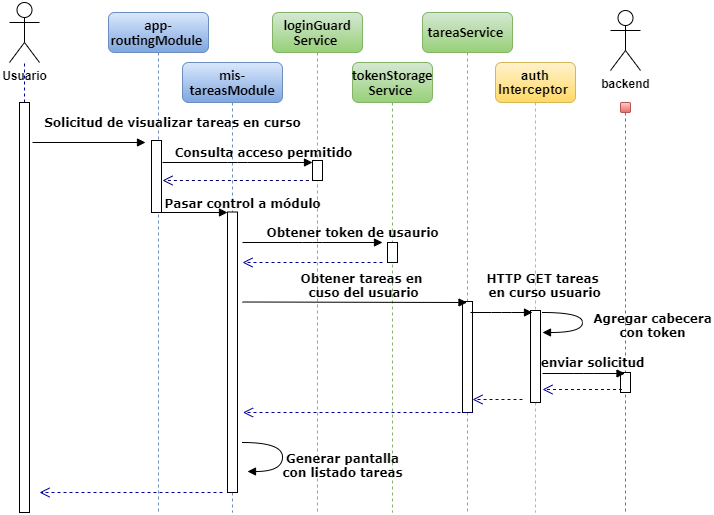
\includegraphics[width=1\textwidth]{./Figures/UsuarioPedidoInteraccion.png}
	\caption{Diagrama de interacción para una solicitud de usuario.}
	\label{fig:UsuarioPedidoInteraccion}
\end{figure}

\pagebreak
\subsubsection{Pantalla principal de vigilancia}

Para el rol de vigilancia se implementó un \textit{WebSocket} que posibilita una comunicación en tiempo real con el backend. Esto permite que ante los intentos de ingreso a planta del personal de tercero, el vigilante pueda tener al instante una alerta, ya sea de un acceso exitoso o de un acceso denegado. Para implementar dicho \textit{WebSocket} se utilizó la librería Socket.io, tanto en el backend como en el frontend. 

A continuación, se muestran los pasos que realiza el sistema y los componentes involucrados en la generación de una alerta:
\begin{enumerate}
\item Cuando el usuario de vigilancia inicia sesión en la aplicación, la misma lo redirige a su página principal (módulo ``homeModule''). En ese momento, el frontend utiliza el servicio ``socketService'' para iniciar el WebSocket con el backend y suscribirse a los eventos de tipo ``ingreso''.
\item Posteriormente, cuando un usuario de tercero intenta ingresar a planta, el backend recibe la solicitud de ingreso, la procesa y genera las tareas de control y alertas correspondientes, según lo explicado en la subsección \ref{sec:subSeccionSolitiudModuloSensor}. Dentro de dichas acciones, el sistema emite un evento del tipo ``ingreso'' que contiene el resultado del intento de acceso, los datos del tercero asociado y una descripción con el motivo de la habilitación o denegación.
\item El módulo ``homeModule'' recibe el evento del backend y genera la alerta al vigilante. La misma se presenta en un \textit{Pop up} que se muestra durante 6 segundos e incluye los detalles del acceso. Para ver el detalle de cada tipo de acceso referirse a la sección \ref{sec:PruebasAceptacion}
\end{enumerate}


\section{Interfaz con sistema de documentación}

El sistema de documentación de terceros es un aplicativo que ya está desarrollado en la empresa. El acceso al mismo es a través de un \textit{endpoint} HTTP GET, al cual se le indica el id del usuario de tercero que se quiere consultar, y devuelve un objeto JSON con la información del nombre y apellido de la persona, si el acceso se debe permitir o no (variable con valor OK o NO) y el motivo por el cual se habilita o no a la mismo. Para configurar el acceso a dicho sistema dentro de nuestro desarrollo, bastó con contar con la dirección del \textit{endpoint}. 

Dado que el desarrollo y las pruebas se realizaron en un entorno desconectado de la empresa, se implementó un \textit{mock} para simular el acceso al sistema. Dicho \textit{mock} se desarrolló como una aplicación web con Node.JS y la librería Express, lo que permitió exponer un \textit{endpoint} HTTP GET del mismo modo que lo hace el sistema original. Para el desarrollo se utilizó el IDE Visual Studio Code y se tomaron 4 casos típicos como respuesta:

\begin{enumerate}
\item Usuario activo con documentación en regla.
\item Usuario activo con documentación vencida.
\item Usuario dado de baja (fin de contratación).
\item Usuario no existente (id de usuario nunca dado de alta).
\end{enumerate}

Con estos 4 casos definidos se pudieron probar todas las alternativas y asegurar la respuesta correcta de nuestra aplicación.

% Chapter Template

\chapter{Ensayos y resultados} % Main chapter title

\label{Chapter4} % Change X to a consecutive number; for referencing this chapter elsewhere, use \ref{ChapterX}

En el presente capítulo se describen las pruebas realizadas sobre el sistema desarrollado y se muestran los resultados obtenidos.


%----------------------------------------------------------------------------------------
%	SECTION 1
%----------------------------------------------------------------------------------------

\section{Detalle de pruebas realizadas}

Para planificar y gestionar todo el proceso de pruebas se desarrolló un \textit{Master Test Plan} \citep{WEBSITE:MasterTestPlan}, donde se especificaron los objetivos de las pruebas, los responsables, la estrategia general y la estrategia por niveles de prueba.   

Los objetivos de las pruebas realizadas sobre el software y hardware fueron:

\begin{itemize}
\item Determinar si el sistema cumple con los requerimientos especificados en la sección \ref{sec:Requerimientos}.
\item Reportar las diferencias entre lo observado y el comportamiento deseado.
\item Dejar evidencias y documentación para probar las siguientes versiones del software y solucionar cualquier \textit{bug} detectado.
\end{itemize}

Para dar cuenta del proceso, en la tabla \ref{tab:tablaTiposPruebas}, se muestra como se organizaron los tipos de prueba realizadas.

\begin{table}[h]
	\centering
	\caption[Tipos de pruebas]{Tipos de pruebas realizadas sobre el sistema.}
	\begin{tabular}{p{3.0cm} p{5.5cm} p{4.0cm}} 	

		\toprule
		\textbf{Tipo de Prueba} & 
		\textbf{Descripción y objetivo } & 
		\textbf{Herramientas utilizadas/Modo de prueba} 
		\\
		\midrule
Pruebas unitarias  &
Este tipo de pruebas permitió verificar de forma separada cada uno de los módulos de hardware y software del sistema. Para aquellos que tenían interfaces con otros módulos se utilizaron \textit{mocks} \citep{WEBSITE:Mocks}, de forma de simular el comportamiento de los mismos sin necesidad de tenerlos implementados.		
		   & Postman/Newman. \textit{mocks} de módulos en caso de ser necesario. \\	
Pruebas de sistema &
Este tipo de prueba permitió verificar el sistema de manera integral, asegurando la correcta comunicación e interrelación de los módulos. &
Pruebas en ambiente de desarrollo sobre el sistema, con los módulos implementados. \\		Pruebas de aceptación &
Este tipo de pruebas permitió validar el sistema de manera integral junto al cliente. De esta forma se aseguró no solo que el sistema se comporte según lo especificado y desarrollado, sino que el usuario final corrobore que el sistema actúa según sus necesidades y requisitos. &
Pruebas en ambiente de desarrollo sobre el sistema, con los módulos implementados.	\\   
		   
		   	
		\bottomrule
		\hline
	\end{tabular}
	\label{tab:tablaTiposPruebas}
\end{table}

Para lograr una trazabilidad entre los requerimientos y los casos de test se implementó, por un lado, una matriz de trazabilidad entre los requerimientos y los casos de uso definidos para el sistema, y por el otro, una matriz de trazabilidad entre los casos de uso y los casos de test. Esto quedó registrado en el documento de Casos de Uso y Casos de Test del sistema \citep{WEBSITE:CasosUsoYTest}.

\pagebreak
\subsection{Herramientas utilizadas}

Para la realización de las pruebas unitarias se utilizó Postman, la cual permitió centralizar y gestionar todas las pruebas desde una única herramienta. Además, se utilizó Newman para automatizar la ejecución de las mismas.

En la figura \ref{fig:Postmanconfig} se muestra la herramienta Postman, junto a la organización de las pruebas unitarias, separadas por módulo y funcionalidad a testear.


\begin{figure}[ht]
	\centering
	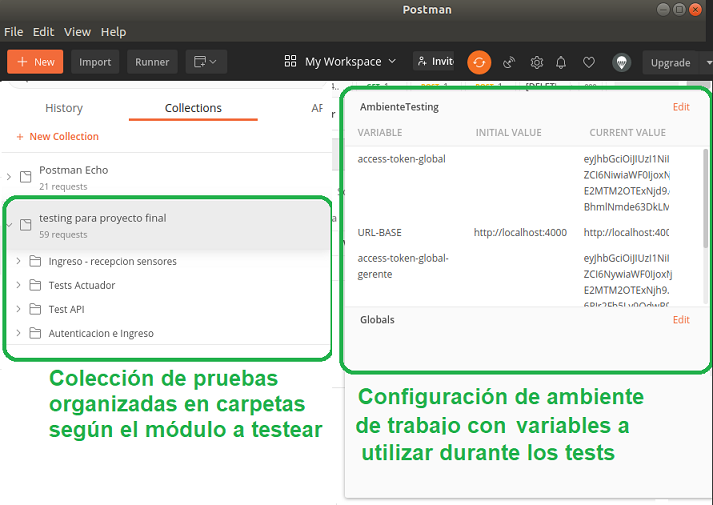
\includegraphics[width=1\textwidth]{./Figures/postman.png}
	\caption{Herramienta Postman junto a su configuración básica.}
	\label{fig:Postmanconfig}
\end{figure}

Por su parte, Newman permite importar los conjuntos de tests definidos en Postman, y mediante un script, ejecutar los mismos y ver los resultados obtenidos. De esta manera podemos correr todos los tests automáticamente, de forma rápida y simple, sin necesidad de hacerlo manualmente.

Para llevar adelante dicho procedimiento, desde Postman se exportaron, tanto la colección de tests, como el ambiente de trabajo (\textit{environment} \citep{WEBSITE:EnvironmentPostman}). Esto generó dos archivos que se utilizaron para configurar la ejecución automática desde Newman. Luego, desarrollamos un script en el backend del trabajo para poder correr la colección con la herramienta de \textit{npm}.

En la figura \ref{fig:scriptNewman} se muestra el script generado y la configuración del mismo en el archivo package.json del módulo de backend.


\begin{figure}[ht]
	\centering
	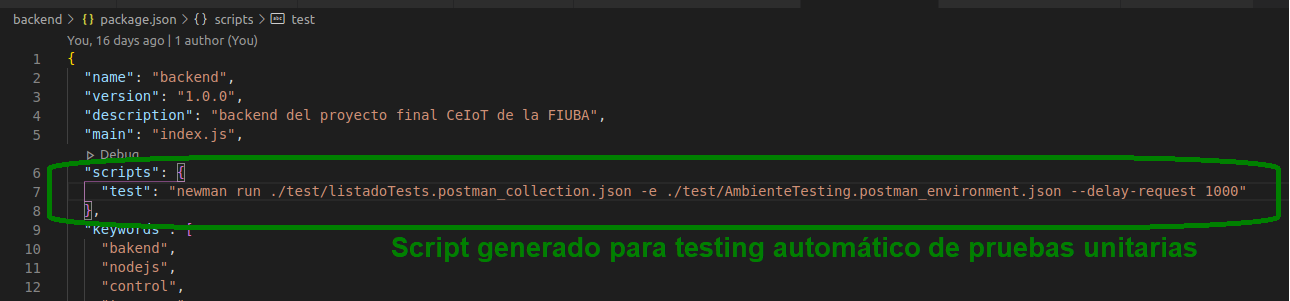
\includegraphics[width=1\textwidth]{./Figures/scriptNewman.png}
	\caption{Configuración del script para testing automático de pruebas unitarias.}
	\label{fig:scriptNewman}
\end{figure}

Por otra parte, en la figura \ref{fig:newmanEjecucion} se muestra la ejecución del script desde la consola de Visual Studio Code y los resultados obtenidos. 


\begin{figure}[ht]
	\centering
	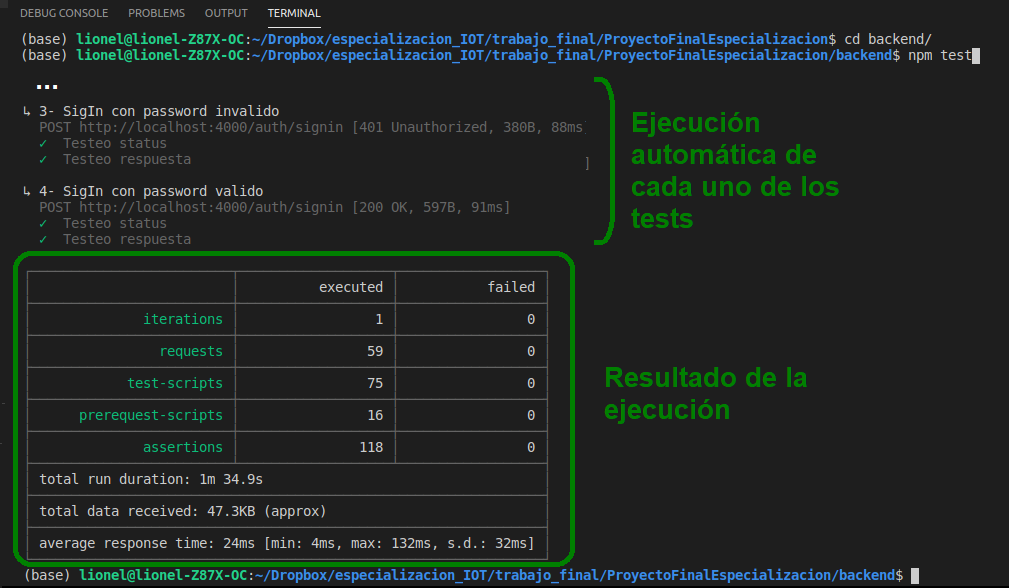
\includegraphics[width=1\textwidth]{./Figures/newmanEjecucion.png}
	\caption{Ejecución y resultados de ejecución del script automático de testing.}
	\label{fig:newmanEjecucion}
\end{figure}


\subsection{Mocks implementados}

Para aquellos módulos que tenían dependencias (interfaces) con otros se utilizaron \textit{mocks}, lo que permitió testearlos, simulando el comportamiento de los dependientes, sin necesidad de tenerlos implementados.

Se desarrollaron dos \textit{mocks} en el trabajo:

\begin{enumerate}
\item mockActuador: este \textit{mock} permitió simular la operatoria del módulo actuador del sistema. El mismo se implementó como una aplicación web en Node.JS que respondía a las peticiones realizadas desde el backend del sistema.
\item mockSistemaTerceros: este \textit{mock} permitió simular la interfaz entre el sistema desarrollado y el sistema de documentación de terceros. El mismo se implementó como una aplicación web en Node.JS, 
\end{enumerate}

    
\pagebreak
\section{Pruebas unitarias}

En esta sección se detalla el conjunto de pruebas unitarias realizadas sobre cada uno de los módulos del sistema.

\subsection{Testing del módulo sensor}

Al momento de testear el módulo sensor, ya se contaba con el módulo del backend desarrollado, con lo cual no fue necesario implementar un \textit{mock}.

Para proceder con las pruebas, se configuraron algunas tarjetas RFID con diferentes valores que simularon cada uno de los escenarios posibles. Se utilizó con tal propósito un programa escrito en Arduino IDE, que permitió asignar el valor a la tarjeta a través del monitor serie. Luego, se alimentó el módulo y se procedió a testear cada caso, acercando una a una las tarjetas ya configuradas para observar los resultados obtenidos.

En la tabla \ref{tab:tablaTestNodSensor} se detalla el conjunto de casos de tests más relevantes implementados para probar el módulo sensor y sus resultados. \footnote{Para tener un detalle completo de los test remitirse al documento de Casos de Uso y Casos de Test del sistema \citep{WEBSITE:CasosUsoYTest}.}

\begin{table}[h]
	\centering
	\caption[Tipos de pruebas sensor]{Casos de test del módulo sensor.}
	\begin{tabular}{p{1.5cm} p{5.5cm} p{5.5cm}} 	

		\toprule
		\textbf{Caso test} & 
		\textbf{Escenario a testear} & 
		\textbf{Resultados} 
		\\
		\midrule
1 & Tarjeta RFID sin valor configurado. & El led de PinTarjNoLeida se prende durante dos segundos y se apaga. \\
2 & Valor de tarjeta RFID recibido correctamente por el backend.	& El led PinOkSistema se prende durante dos segundos y se apaga. \\
3 & El módulo sensor no registrado en el sistema. & El led PinNoOkSistemaCodigo se prende durante dos segundos y se apaga. \\
4 & El módulo sensor no está activo en el sistema. & El led PinNoOkSistemaCodigo se prende durante dos segundos y se apaga. \\	   
		\bottomrule
		\hline
	\end{tabular}
	\label{tab:tablaTestNodSensor}
\end{table}

En la figura \ref{fig:TestTajetaSinCodigo} se muestra el caso de test 1 donde la tarjeta no tiene valor configurado. En la primera imagen se ve el momento en que se acerca la tarjeta y en la segunda imagen se ve el momento en que el módulo responde al usuario.


\begin{figure}[ht]
	\centering
	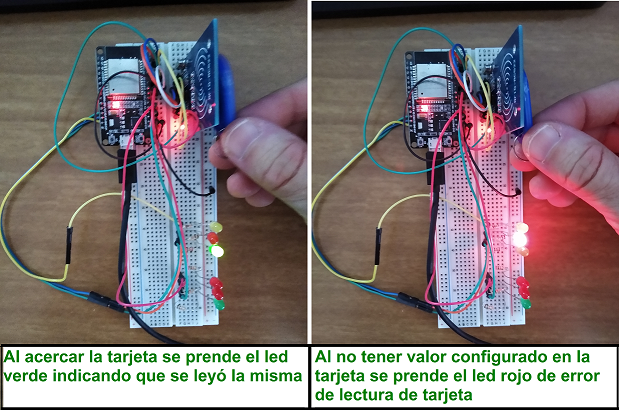
\includegraphics[width=0.8\textwidth]{./Figures/TestTajetaSinCodigo.png}
	\caption{Procedimiento de prueba para el caso de test 1 con tarjeta sin valor configurado.}
	\label{fig:TestTajetaSinCodigo}
\end{figure}

\clearpage
En la figura \ref{fig:TestTajetaCodigoLeida} se muestra el caso de test 2 donde la tarjeta es válida, y el sistema se comunica correctamente con el módulo del backend. En la primera imagen se ve el momento en que se acerca la tarjeta y en la segunda imagen se ve el momento en que el módulo responde al usuario.


\begin{figure}[ht]
	\centering
	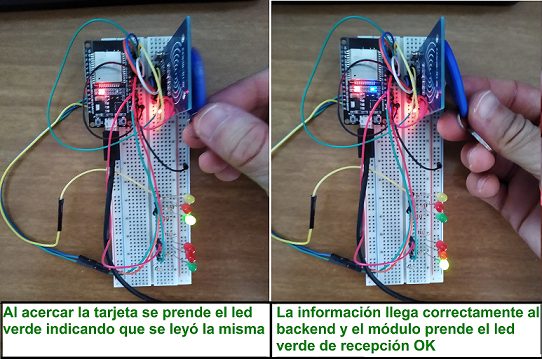
\includegraphics[width=0.8\textwidth]{./Figures/TestTajetaCodigoLeida.png}
	\caption{Procedimiento de prueba para el caso de test 2 con tarjeta con valor configurado y recibido correctamente por el backend.}
	\label{fig:TestTajetaCodigoLeida}
\end{figure}



\subsection{Testing del módulo actuador}

Para testear el módulo actuador se utilizó Postman, dado que el módulo expone una conexión HTTP POST. Dentro de Postman generamos una carpeta llamada Test Actuador, en la cual almacenamos todos los casos de test. En el \textit{body} se envían los valores como un objeto JSON.

En la figura \ref{fig:TestActuadorConfig} se muestra la configuración de Postman para el testeo del módulo actuador.

\begin{figure}[ht]
	\centering
	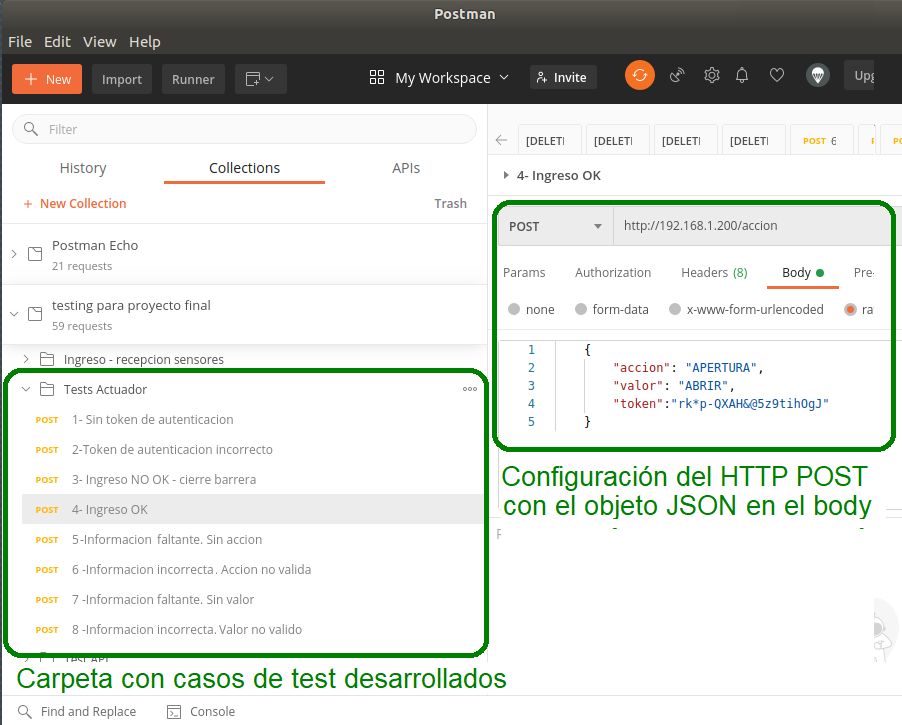
\includegraphics[width=0.9\textwidth]{./Figures/TestActuadorConfig.png}
	\caption{Configuración en Postman para el testeo del módulo actuador.}
	\label{fig:TestActuadorConfig}
\end{figure}

La prueba implicó testear cada uno de los casos generados, ejecutándolos desde Postman. A fin de automatizar los tests, y no depender de un control manual de la respuesta obtenida luego de cada ejecución, se configuraron para cada test las condiciones esperadas o aserciones, utilizando la sección Tests de la herramienta. Algunas de las aserciones definidas fueron que el código de estado HTTP sea el esperado y/o que la respuesta contenga cierto dato o cierto objeto JSON con determinados valores. Al ejecutar el test, si los resultados eran los previstos, Postman indicaba en el apartado Test Results que los mismos eran correctos.

En la figura \ref{fig:PostmanAsercion} se muestra un ejemplo de configuración de la sección Tests y la ejecución del caso de test.

\begin{figure}[ht]
	\centering
	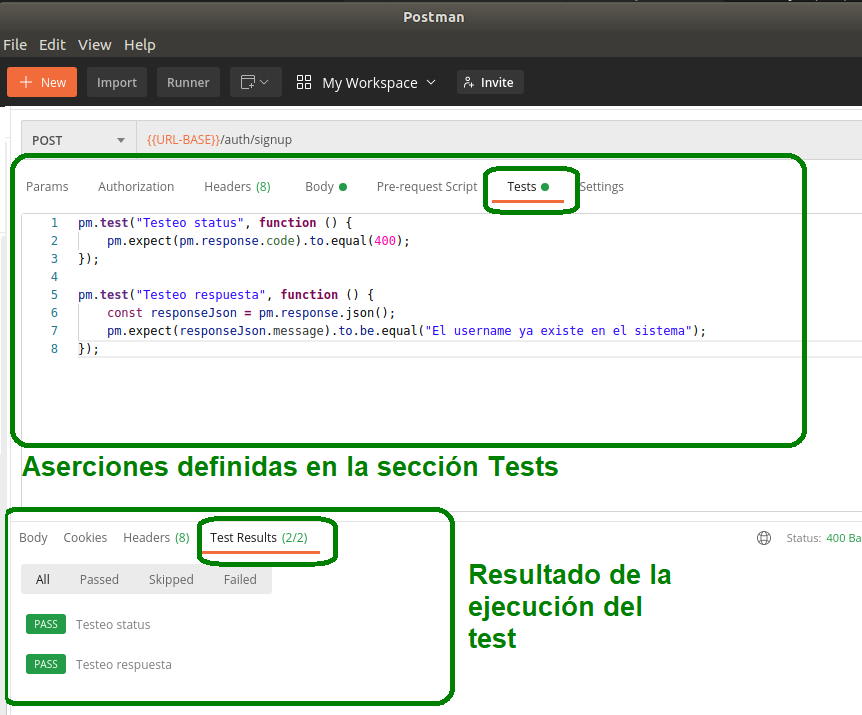
\includegraphics[width=0.8\textwidth]{./Figures/PostmanAsercion.png}
	\caption{Configuración de sección Tests y resultados de la ejecución del test.}
	\label{fig:PostmanAsercion}
\end{figure}

En la tabla  \ref{tab:tablaTestNodActuador} se detalla el conjunto de casos de tests más relevantes implementados para probar el módulo actuador y sus resultados. Dentro del escenario a testear entre paréntesis se hace referencia al nombre del test en Postman. \footnote{Para tener un detalle completo de los test remitirse al documento de Casos de Uso y Casos de Test del sistema \citep{WEBSITE:CasosUsoYTest}.}


\begin{table}[h]
	\centering
	\caption[Tipos de pruebas actuador]{Casos de test del módulo actuador.}
	\begin{tabular}{p{1.5cm} p{6.5cm} p{4.5cm}} 	

		\toprule
		\textbf{Caso test} & 
		\textbf{Escenario a testear} & 
		\textbf{Resultados} 
		\\
		\midrule
1 & Habilitar ingreso a la planta (Ingreso OK). & El led IngresoOk parpadea durante 4 segundos y se activa la cerradura. \\
2 & Inhabilitar ingreso a la planta (Ingreso NO OK – cierre barrera).	& El led IngresoNOOk se prende durante dos segundos y se apaga. \\
3 & El pedido HTTP POST no cuenta con el campo de acción a realizar (Información faltante – Acción no válida). & El led Error parpadea dos veces. \\
4 & El pedido HTTP POST no cuenta con token de autenticación (Sin token de autenticación). & El led Error parpadea una vez. \\	   
		\bottomrule
		\hline
	\end{tabular}
	\label{tab:tablaTestNodActuador}
\end{table}




En la sección \ref{sec:PruebasAceptacion} se muestra el detalle de los casos de ingreso habilitado e inhabilitado junto a una figura del módulo actuador. Remitirse a dicha sección para más detalles.


\subsection{Testing del módulo de backend}

Para testear el módulo de backend se utilizó Postman, dado que el módulo expone una API Rest al frontend, una API de autenticación y un \textit{endpoint} \citep{WEBSITE:Endpoints} para recibir los datos de los módulos sensores. Dentro de Postman generamos una carpeta llamada Test API para testear la API expuesta al frontend, una carpeta llamada Autenticación e ingreso para testear la API de autenticación y una carpeta llamada Ingreso – recepción sensores para testear los ingresos generados desde el módulo sensor.

Dentro de la carpeta de Test API generamos cuatro subcarpetas para testear los casos sin autenticación y con autenticación para los diferentes perfiles de usuario. Dentro de la carpeta de Autenticación e ingreso, se colocaron los tests para el alta de usuario y el ingreso al sistema. Y dentro de la capeta Ingreso – recepción sensores, los tests para los ingresos generados desde el módulo sensor.

En la figura \ref{fig:testsBackend} se muestra las carpetas configuradas en Postman para el testeo de los casos de test de backend.

\begin{figure}[h]
	\centering
	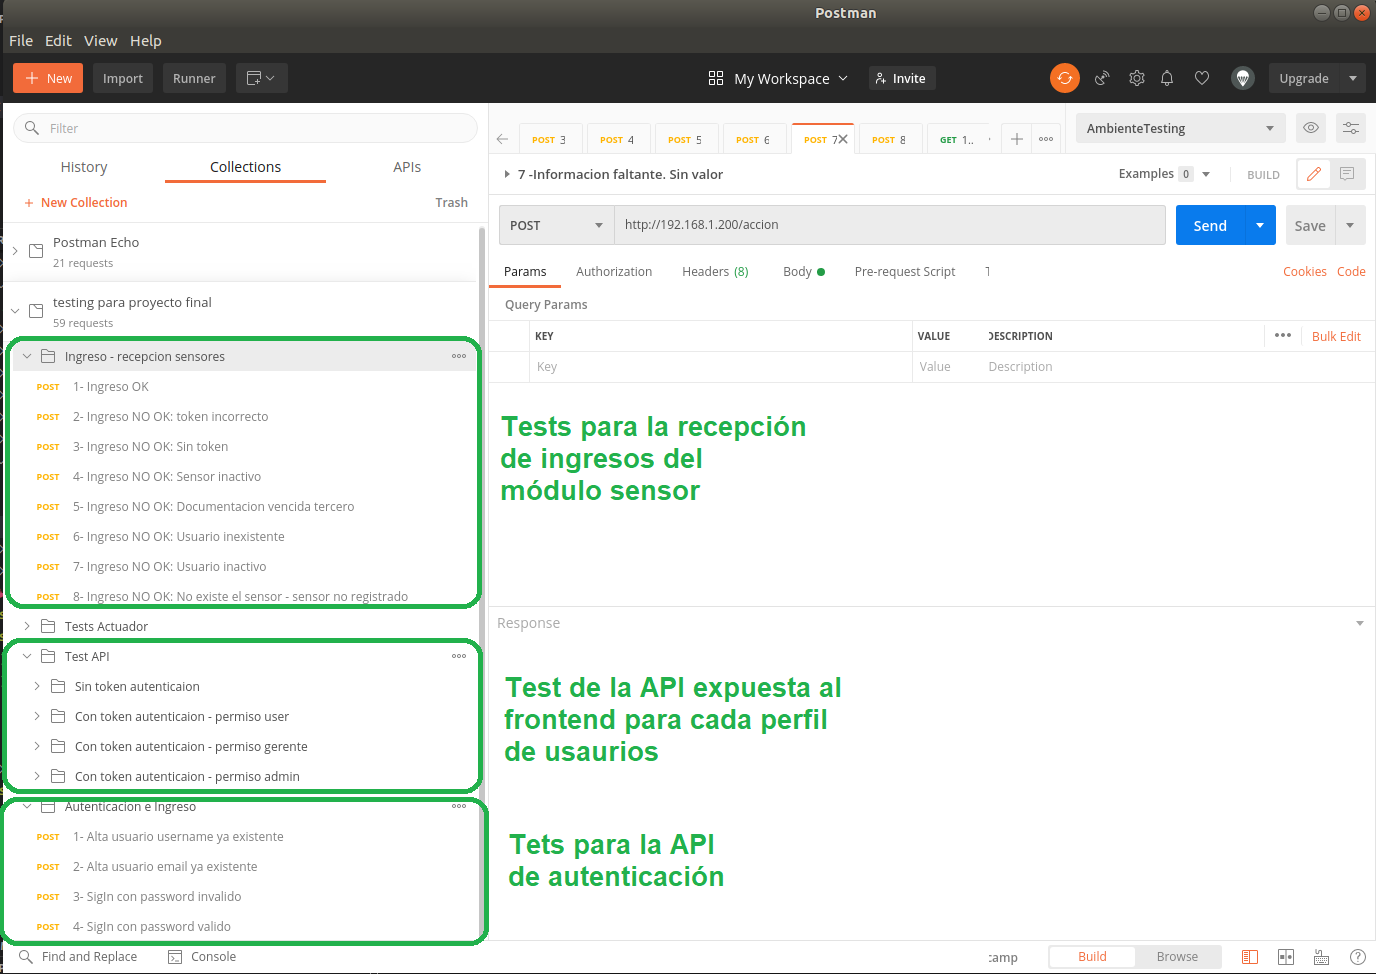
\includegraphics[width=1\textwidth]{./Figures/testsBackend.png}
	\caption{Configuración en Postman para el testeo del módulo de backend.}
	\label{fig:testsBackend}
\end{figure}


Para testear cada caso, se procedió a configurar en Postman la URL de cada \textit{endpoint}, junto a los parámetros requeridos. Para los pedidos HTTP GET se configuró directamente la URL con los parámetros, y para los HTTP POST se completó el \textit{body} con el objeto JSON, junto a los valores requeridos según cada caso. 

\pagebreak
Para los casos de test con autenticación definidos dentro de la carpeta Test API, se procedió a utilizar los \textit{environments} y las variables globales de Postman. Un \textit{environment} permite definir ambientes de testing, dentro de los cuales podemos definir variables globales que pueden utilizarse en varios tests. Un test puede obtener un valor de la respuesta HTTP y guardarlo en una variable global, para luego ser utilizado por otro. De este modo, definimos un \textit{environment} llamado AmbienteTesting y dentro del mismo configuramos las siguientes variables globales:

\begin{itemize}
\item URL-BASE: contiene la URL base del backend a partir del cual se define cada \textit{endpoint}. Con la misma configuramos cada HTTP POST o GET, de modo que si cambia la URL de nuestro backend, con solo modificar esta variable quedan ajustados todos los \textit{endpoints}.

\item Access-token-global: utilizado para los \textit{endpoints} que son accesibles para cualquier usuario del sistema. Permite guardar el token de acceso del rol usuario.

\item Access-token-global-gerente: utilizado para los \textit{endpoints} que son accesibles solo por el perfil de gerente de la aplicación. Permite guardar el token de acceso de rol gerente.

\item Access-token-global-admin: utilizado para los \textit{endpoints} que son accesibles solo por el perfil de administrador de la aplicación. Permite guardar el token de acceso para el rol de administrador.
\end{itemize}

Los tokens de acceso se configuran dentro de la sección header del test, con clave x-access-token y con el valor del token.

En la figura \ref{fig:PostmanEnvironmnet} se muestra las variables globales definidas en Postman.

\begin{figure}[ht]
	\centering
	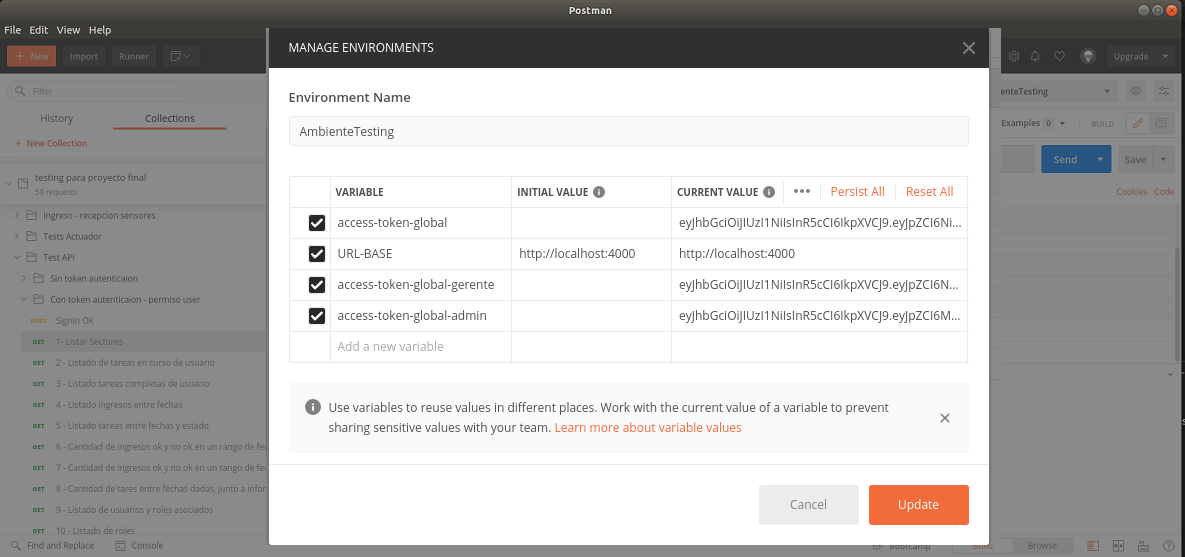
\includegraphics[width=1\textwidth]{./Figures/PostmanEnvironmnet.png}
	\caption{Variables globales definidas en Postman.}
	\label{fig:PostmanEnvironmnet}
\end{figure}

\subsubsection{Tests de carpeta Test API }

Dentro de la carpeta Test API tenemos cuatro subcarpetas:

\begin{itemize}
\item Sin token autenticación: testea los \textit{endpoints} sin un token de autenticación.
\item Con token autenticación – permiso user: testea los \textit{endpoints}  que son accesibles para cualquier usuario del sistema. En esta carpeta se define un test inicial llamado SigIn OK, que se utilizó para simular la autenticación de un usuario normal y completar la variable global access-token-global que fue utilizada por el resto de los tests de la carpeta.
\item Con token autenticación – permiso gerente: testea los \textit{endpoints}  que son accesibles para el usuario con rol gerente. En esta carpeta se define un test inicial llamado SigIn OK, que se utilizó para simular la autenticación de un usuario gerente y completar la variable global access-token-global-gerente que fue utilizada por el resto de los tests de la carpeta.
\item Con token autenticación – permiso admin: testea los \textit{endpoints} que son accesibles para el usuario con rol administrador. En esta carpeta se define un test inicial llamado SigIn OK, que se utilizó para simular la autenticación de un usuario administrador y completar la variable global access-token-global-admin que fue utilizada por el resto de los tests de la carpeta.
\end{itemize}

En la figura \ref{fig:TestBackendGerente} se muestran los tests de la subcarpeta Con token autenticación – permiso gerente, junto al test inicial de SignIn OK y al resto de los tests.

\begin{figure}[ht]
	\centering
	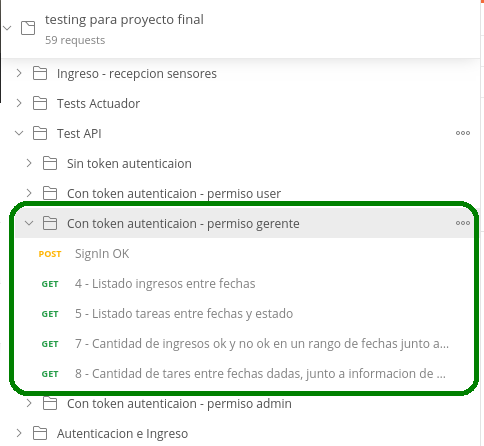
\includegraphics[width=0.7\textwidth]{./Figures/TestBackendGerente.png}
	\caption{Tests de la subcarpeta Con token autenticación – permiso gerente.}
	\label{fig:TestBackendGerente}
\end{figure}

\pagebreak
\subsubsection{Detalle de tests y resultados}

En la tabla  \ref{tab:tablaTestBackendSensor} se detalla el conjunto de casos de tests más relevantes implementados para probar la recepción de los datos de los módulos sensores y sus resultados. En la columna escenario a testear se hace referencia, entre paréntesis, al número del test en Postman.  \footnote{Para tener un detalle completo de los test remitirse al documento de Casos de Uso y Casos de Test del sistema \citep{WEBSITE:CasosUsoYTest}.}


\begin{table}[h]
	\centering
	\caption[Tipos de pruebas backend]{Casos de test del módulo backend. Testing de recepción de los datos de los módulos sensores.}
	\begin{tabular}{p{3.5cm} p{4.5cm} p{4cm}} 	

		\toprule
		\textbf{Subcarpeta Postman} & 
		\textbf{Escenario a testear} &
		\textbf{Resultados} 
		\\
		\midrule

 Ingreso – recepción sensores.                  
& Ingreso con valor de tarjeta registrado en el sistema y módulo sensor activo (1).
& Se confirma recepción con HTTP código 200.  \\
& El módulo sensor no está registrado en el sistema  (8).
& Se rechaza el ingreso con mensaje de error de sensor inexistente. \\
& El módulo sensor no está activo en el sistema (4). 
& Se rechaza el ingreso con mensaje de error de sensor inactivo. \\
		\bottomrule
		\hline
	\end{tabular}
	\label{tab:tablaTestBackendSensor}
\end{table}


En la tabla \ref{tab:tablaTestBackendFrontend} se detalla el conjunto de casos de tests más relevantes implementados para probar la API Rest expuesta al frontend y sus resultados. En la columna escenario a testear se hace referencia, entre paréntesis, al número del test en Postman.  \footnote{\label{notaReusadaCasosTest}Para tener un detalle completo de los test remitirse al documento de Casos de Uso y Casos de Test del sistema \citep{WEBSITE:CasosUsoYTest}.}


\begin{table}[h]
	\centering
	\caption[Tipos de pruebas backend]{Casos de test del módulo backend. Testing de la API Rest expuesta al frontend.}
	\begin{tabular}{p{3.5cm} p{3.5cm} p{5cm}} 	

		\toprule
		\textbf{Subcarpeta Postman} & 
		\textbf{Escenario a testear} &
		\textbf{Resultados} 
		\\
		\midrule

\multirow{2}{3.5cm}{Test API/Sin token autenticación.} & Listar sectores de la empresa (1). & Se acepta el pedido y se devuelve el listado de sectores de la empresa. \\
                    & Resto de los \textit{endpoints}. & Se rechaza el pedido por falta de token de autenticación con un HTTP 403. \\
\hline
\multirow{3}{3.5cm}{Test API/Con token autenticación – permiso user.} & Listado de tareas en curso del usuario (2). & Se acepta el pedido y se devuelve el listado de tareas en curso del usuario. \\
                    & Listado de tareas completas del usuario (3). & Se acepta el pedido y se devuelve el listado de tareas completas del usuario. \\
                    & Cantidad ingresos a la empresa por día (7). & Se rechaza el pedido por no tener rol gerente o administrador con un HTTP 403. \\
\hline
\multirow{2}{3.5cm}{Test API/Con token autenticación – permiso gerente.}  & Cantidad ingresos a la empresa por día (7). & Se acepta el pedido y se devuelve el listado de ingresos OK y no OK para las fechas indicadas. \\
                    & Listado detalle de tareas en curso entre rango de fechas (5). & Se acepta el pedido y se devuelve el listado de tareas y sub-tareas para las fechas indicadas. \\
\hline
\multirow{2}{3.5cm}{Test API/Con token autenticación – permiso admin.}  & Listado de usuarios y roles (9). & Se acepta el pedido y se devuelve el listado de usuarios y roles de cada usuario. \\
                    & Cambiar estado de rol de usuario (12). & Se acepta el pedido y ajusta el estado del rol para el usuario indicado. \\
		\bottomrule
		\hline
	\end{tabular}
	\label{tab:tablaTestBackendFrontend}
\end{table}

\pagebreak
En la tabla  \ref{tab:tablaTestBackendAutenticacion} se detalla el conjunto de casos de tests más relevantes implementados para probar la API de autenticación y sus resultados. En la columna escenario a testear se hace referencia, entre paréntesis, al número del test en Postman.


\begin{table}[h]
	\centering
	\caption[Tipos de pruebas backend]{Casos de test del módulo backend. Testing de la API de autenticación.}
	\begin{tabular}{p{3.5cm} p{4.5cm} p{4cm}} 	

		\toprule
		\textbf{Subcarpeta Postman} & 
		\textbf{Escenario a testear} &
		\textbf{Resultados} 
		\\
		\midrule
\multirow{3}{3.5cm}{Autenticación e ingreso.} & Alta de usuario con username, email y password correcto (5). & Se confirma el alta del usuario con HTTP código 200. \\
                    & Alta de usuario con username o email repetido (1 y2). & Se rechaza el alta. Respuesta HTTP con código 400 y mensaje de error. \\
                    & Inicio de sesión con username o password incorrecto (3 y 4). & Se rechaza el inicio de sesión. Respuesta HTTP con código 401 y mensaje de error. \\
		\bottomrule
		\hline
	\end{tabular}
	\label{tab:tablaTestBackendAutenticacion}
\end{table}


\section{Pruebas de sistema}

En esta sección se detalla el conjunto de pruebas integrales realizadas sobre el sistema con todos sus módulos. Este test fue ejecutado por el desarrollador en el ambiente de pruebas, sin el cliente.

Una vez implementados todos los módulos del sistema, fueron realizadas las siguientes tareas:

\begin{enumerate}
\item Se crearon usuarios con cada uno de los roles en la base de datos.
\item Se alimentó el módulo sensor y el módulo actuador.
\item Se corrió el módulo de backend, el \textit{mock} del sistema de terceros y el módulo de frontend. Con el propósito de automatizar este paso, se desarrolló un script para ejecutar y levantar los módulos antes mencionados, mediante el uso de contenedores \textit{Docker} y de la herramienta \textit{docker-compose}. 

\end{enumerate}

Con los módulos en ejecución, se procedió a \textit{loguearse} en el sistema. En primer lugar, con un rol de usuario normal, luego con el rol de usuario gerente, posteriormente con el rol vigilante y por último con el rol administrador.

En la tabla  \ref{tab:tablaTestsSistemaUsuNormal} se detalla el conjunto de casos de tests más relevantes implementados para probar el rol de usuario normal del sistema y los resultados obtenidos.\footnote{\label{notaReusadaCasosTest}Para tener un detalle completo de los test remitirse al documento de Casos de Uso y Casos de Test del sistema \citep{WEBSITE:CasosUsoYTest}.}

\begin{table}[h]
	\centering
	\caption[Tipos de pruebas sistema]{Listado de pruebas de sistemas realizadas para el rol de usuario normal.}
	\begin{tabular}{ p{4cm} p{8.5cm}} 	

		\toprule
		\textbf{Pantalla del sistema testeada/Acción} & 
		\textbf{Resultados} 
		\\
		\midrule
Mis tareas en curso/Visualizar tareas.  & El sistema muestra el listado de tareas en curso del usuario o indica que no tiene tareas en curso. \\
Mis tareas en curso/Cerrar tarea.  & El sistema marca como completa la tarea del usuario y  muestra una alerta indicando que se cerró la tarea correctamente.  \\
Mis tareas en curso/Ajustar observación en tarea.  & El sistema ajusta la observación en la tarea y muestra una alerta indicando que se actualizó la observación correctamente. \\
Mi historial tareas/Visualizar historial tareas de usuario. & El sistema muestra el listado de tareas cerradas del usuario o indica que no tiene tareas cerradas. \\
Mi perfil/Visualizar perfil. & El sistema muestra la información del usuario, incluyendo su \textit{username}, email, sector y roles asignados. \\

		\bottomrule
		\hline
	\end{tabular}
	\label{tab:tablaTestsSistemaUsuNormal}
\end{table}


En la tabla  \ref{tab:tablaTestsSistemaUsuAdmin} se detalla el conjunto de casos de tests más relevantes implementados para probar el rol de usuario administrador del sistema y los resultados obtenidos. 

\begin{table}[h]
	\centering
	\caption[Tipos de pruebas sistema]{Listado de pruebas de sistemas realizadas para el rol de usuario administrador.}
	\begin{tabular}{ p{4cm} p{8.5cm}} 	

		\toprule
		\textbf{Pantalla del sistema testeada/Acción} & 
		\textbf{Resultados} 
		\\
		\midrule
Gestión usuarios/Modificar estado de rol de usuario.  & El sistema modifica el estado del rol del usuario en la base de datos y muestra una alerta indicando que el cambio se realizó correctamente.  \\
		\bottomrule
		\hline
	\end{tabular}
	\label{tab:tablaTestsSistemaUsuAdmin}
\end{table}

En la tabla  \ref{tab:tablaTestsSistemaUsuPorteria} se detalla el conjunto de casos de tests más relevantes implementados para probar el rol de usuario vigilante del sistema y los resultados obtenidos. 

\begin{table}[h]
	\centering
	\caption[Tipos de pruebas sistema]{Listado de pruebas de sistemas realizadas para el rol de usuario vigilante.}
	\begin{tabular}{ p{4cm} p{8.5cm}} 	

		\toprule
		\textbf{Pantalla del sistema testeada/Acción} & 
		\textbf{Resultados} 
		\\
		\midrule
Pantalla principal/Visualizar ingreso en portería.  & Cuando un tercero pretende ingresar en planta, el sistema muestra en su pantalla principal una alerta, indicando el intento de acceso y si el mismo se permitió o se rechazó, junto a un color particular para diferenciar ambos casos. La alerta se muestra por 6 segundos. \\
		\bottomrule
		\hline
	\end{tabular}
	\label{tab:tablaTestsSistemaUsuPorteria}
\end{table}


En la tabla  \ref{tab:tablaTestsSistemaUsuGerente} se detalla el conjunto de casos de tests más relevantes implementados para probar el rol de usuario gerente del sistema y los resultados obtenidos. 

\begin{table}[h]
	\centering
	\caption[Tipos de pruebas sistema]{Listado de pruebas de sistemas realizadas para el rol de usuario gerente.}
	\begin{tabular}{ p{4cm} p{8.5cm}} 	

		\toprule
		\textbf{Pantalla del sistema testeada/Acción} & 
		\textbf{Resultados} 
		\\
		\midrule
Estadísticas ingresos/Visualizar ingresos del mes.  & El sistema muestra un gráfico de barras con la cantidad de ingresos de cada día del mes especificado (ingresos ok y no ok) y un gráfico de torta con el total de ingresos ok y no ok del mes.  \\
Estadísticas tareas/Visualizar estadísticas de tareas.  & El sistema muestra un gráfico de torta con la cantidad de tareas en curso, un gráfico de barras con la cantidad de tareas cerradas por cada mes del año y un gráfico de torta con el total de tareas completas del año.  \\
Tareas en curso/Visualizar tareas en curso.
  & El sistema muestra el listado de tareas en curso, junto a información de antigüedad, estado, fecha de inicio y detalle de las sub-tarea de cada sector.  \\
Ingresos del día/Visualizar ingresos del día.  & El sistema muestra el listado de los ingresos, junto a información de horario, si el ingreso fue permitido o no y el detalle de la habilitación o rechazo junto al nombre del tercero.  \\

		\bottomrule
		\hline
	\end{tabular}
	\label{tab:tablaTestsSistemaUsuGerente}
\end{table}


\pagebreak
\section{Pruebas de aceptación}\label{sec:PruebasAceptacion}

En esta sección se detallan dos de las pruebas de aceptación realizadas en conjunto con el cliente. Estos tests fueron llevados a cabo por el desarrollador del sistema, en el ambiente de pruebas, para verificar el funcionamiento correcto del sistema implementado.

Para preparar dicho ambiente se procedió de igual modo que el descripto en la sección anterior para las pruebas de sistema.

\subsection{Descripción y detalles de prueba de ingreso habilitado}

En esta sección se detalla la prueba de ingreso de un tercero a la empresa que cuenta con la documentación requerida en regla.

Para realizar la prueba se preparó el sistema y se lo dejó operativo. Se utilizó la tarjeta RFID de un tercero que estaba habilitado y un usuario con rol de vigilancia generado previamente.

A continuación, se detallan los pasos realizados para el caso descripto:

\begin{enumerate}
\item Se ingresó al sistema con el usuario Portería y se accedió a la página principal.
\item Se tomó la tarjeta RFID del personal de tercero habilitado en el sistema y se la acercó al módulo sensor. Como respuesta a esta interacción, sucedieron las siguientes acciones:

	\begin{enumerate}
	\item El módulo sensor prendió el led verde de lectura de la tarjeta y luego prendió el led verde de comunicación correcta con el sistema de control.
	\item En la pantalla del usuario de portería se visualizó la alerta de ingreso del tercero durante 6 segundos. A continuación, se corroboró que el contador de ingresos correctos se había incrementado en la pantalla.
	\item El módulo actuador prendió de forma intermitente el led verde de ingreso habilitado durante 4 segundos y se cerró el pestillo de la cerradura electrónica. Pasado ese tiempo el pestillo se abrió nuevamente.
	\end{enumerate}


\end{enumerate}

En la figura \ref{fig:TestTajetaCodigoLeida2} se muestra el paso 2 de la prueba con el acercamiento de la tarjeta RFID al módulo sensor y la respuesta de dicho módulo.

\vspace{1cm}
\begin{figure}[h]
	\centering
	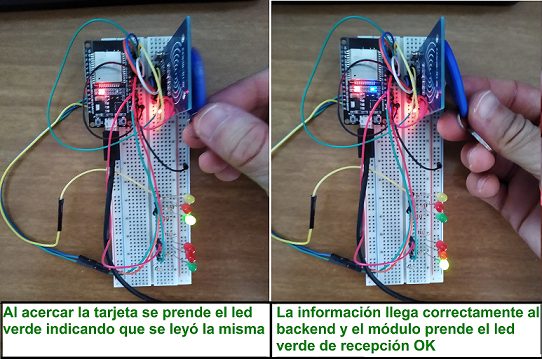
\includegraphics[width=1\textwidth]{./Figures/TestTajetaCodigoLeida.png}
	\caption{Accionamiento de módulo sensor con tarjeta RFID y respuesta del módulo.}
	\label{fig:TestTajetaCodigoLeida2}
\end{figure}

En la figura \ref{fig:ingresoOk} se muestra el paso 2 b) de prueba con la información visualizada por la vigilancia.

\begin{figure}[h]
	\centering
	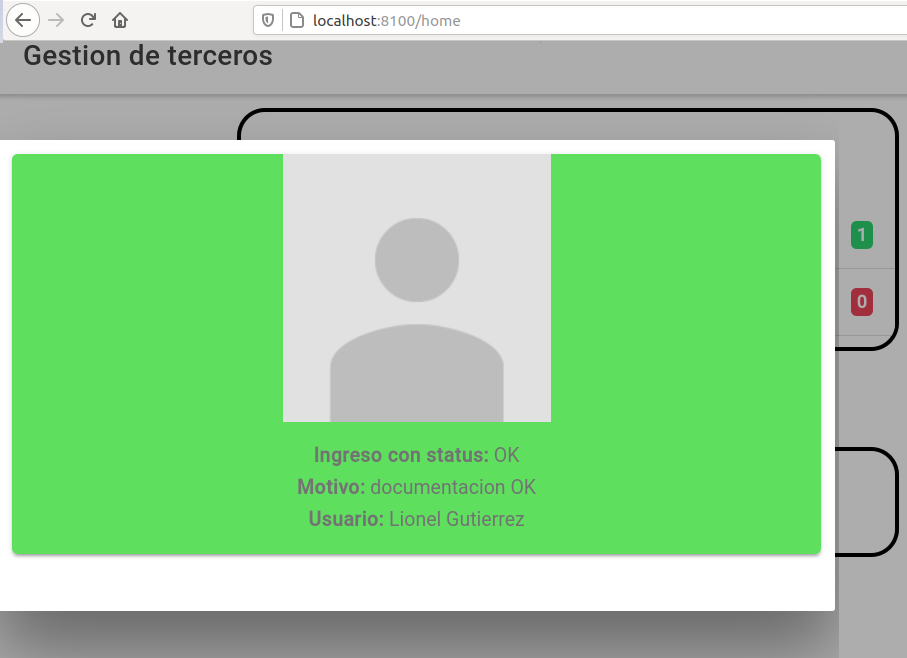
\includegraphics[width=1\textwidth]{./Figures/ingresoOk.png}
	\caption{Visualización de la alerta recibida en pantalla.}
	\label{fig:ingresoOk}
\end{figure}

En la figura \ref{fig:actuadorOK} se muestra el paso 2 c) de la prueba, donde se ve el módulo actuador con el led prendido y el pestillo de la cerradura cerrada.

\begin{figure}[h]
	\centering
	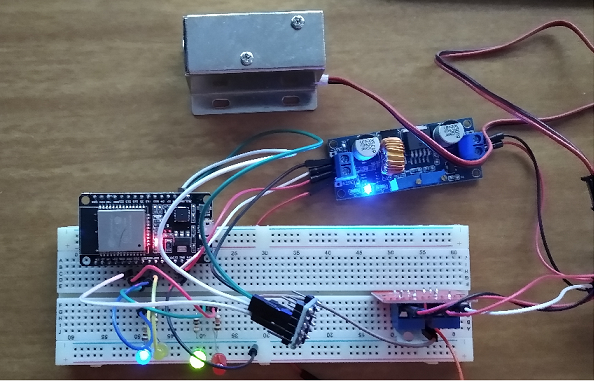
\includegraphics[width=1\textwidth]{./Figures/actuadorOK.png}
	\caption{Accionamiento de módulo actuador y respuesta del módulo.}
	\label{fig:actuadorOK}
\end{figure}

\clearpage
\subsection{Descripción y detalles de prueba de ingreso inhabilitado}

En esta sección se detalla la prueba de ingreso de un tercero a la empresa que no cuenta con la documentación requerida en regla.

Para realizar la prueba se preparó el sistema y se lo dejó operativo. Se utilizó la tarjeta RFID de un tercero que tenía problemas con su documentación y un usuario con rol de vigilancia generado previamente.

A continuación, se detallan los pasos realizados para el caso descripto:

\begin{enumerate}
\item Se ingresó al sistema con el usuario Portería y se accedió a la página principal.
\item Se tomó la tarjeta RFID del personal de tercero inhabilitado en el sistema y se acercó la misma al módulo sensor. Como respuesta a esta interacción, sucedieron las siguientes acciones:

	\begin{enumerate}
	\item El módulo sensor prendió el led verde de lectura de la tarjeta y luego prendió el led verde de comunicación correcta con el sistema de control.
	\item En la pantalla del usuario de portería se visualizó la alerta de ingreso inhabilitado del tercero durante 6 segundos. A continuación, se corroboró que el contador de intento de ingresos incorrectos se había incrementado en la pantalla.
	\item El módulo actuador prendió durante 2 segundos el led rojo de ingreso inhabilitado. El pestillo de la cerradura electrónica se mantuvo abierto todo el tiempo.
	\item Se envió un email a los usuarios de los sectores encargados de controlar la documentación del tercero, con el detalle del intento de ingreso.
	\item Se generó una tarea de control de documentación para cada uno de los sectores de la empresa responsables del proceso.
	\end{enumerate}

\item Se ingresó al sistema con un usuario de sector HESA (Seguridad y Medio Ambiente) para corroborar la generación de la tarea de control. Se accedió a la aplicación Mis tareas en curso (preguntar como pongo estas cosas) y se visualizó la nueva tarea asignada al usuario.
\end{enumerate}

En la figura \ref{fig:ingresNOOK} se muestra el paso 2 b) de la prueba con la información visualizada por la vigilancia.

\begin{figure}[ht]
	\centering
	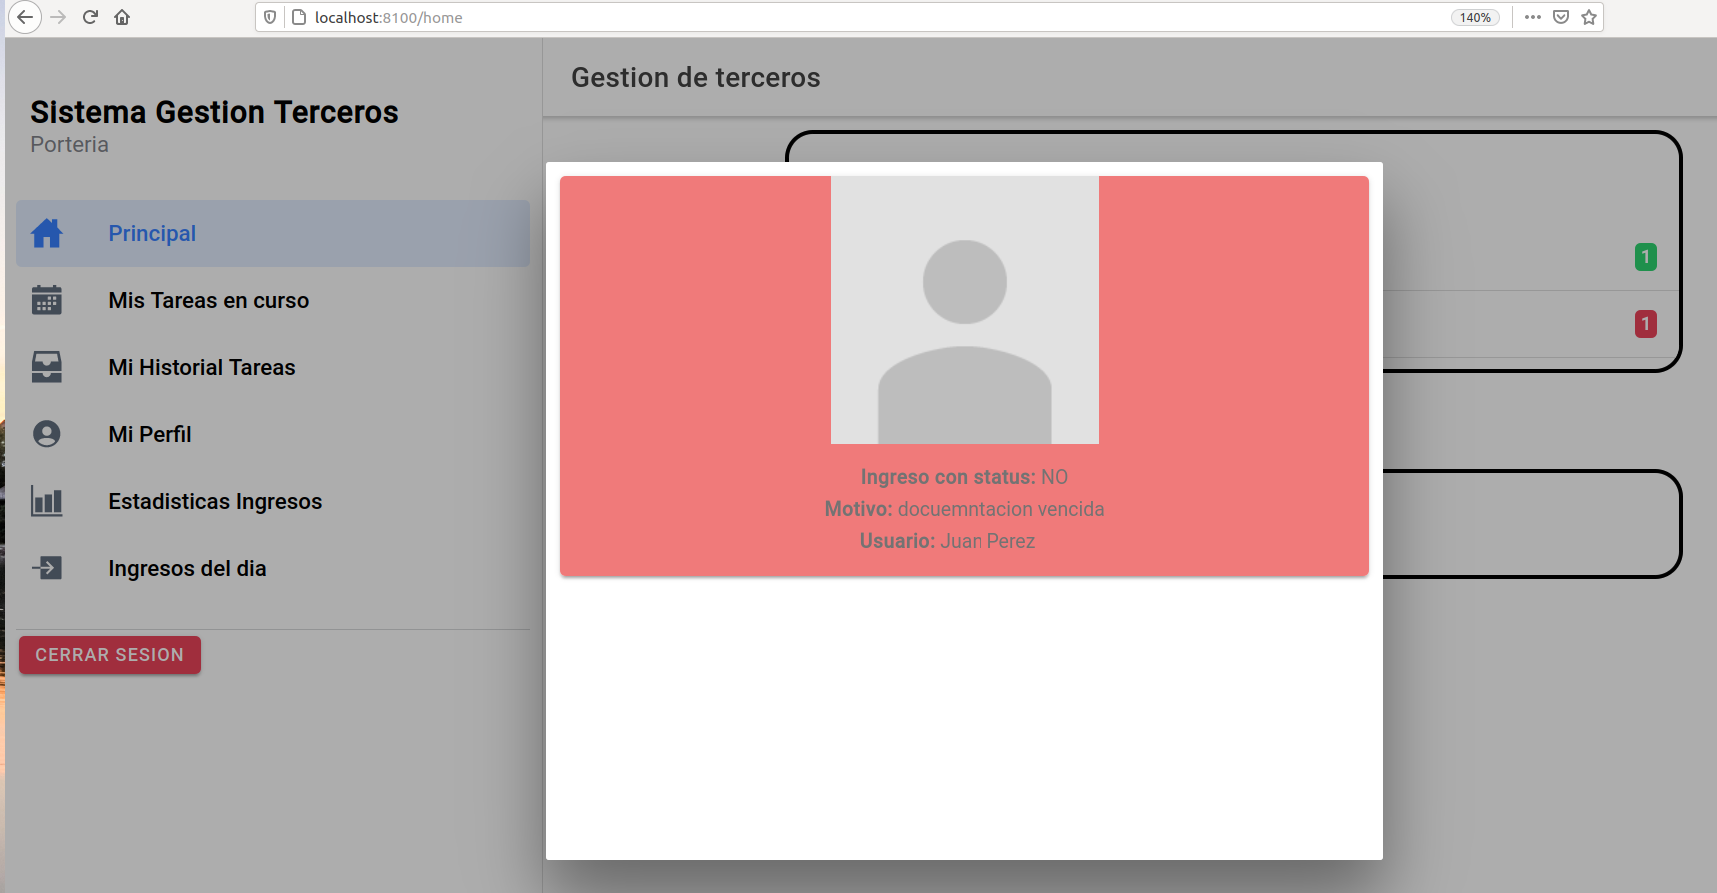
\includegraphics[width=1\textwidth]{./Figures/ingresoNOOK.png}
	\caption{Visualización de la alerta recibida en pantalla.}
	\label{fig:ingresNOOK}
\end{figure}

En la figura \ref{fig:actuadorNOOK} se muestra el paso 2 c) de la prueba, donde se ve el módulo actuador con el led rojo prendido y el pestillo de la cerradura abierta.

\begin{figure}[ht]
	\centering
	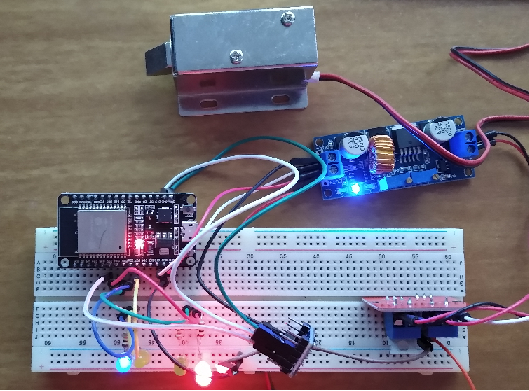
\includegraphics[width=1\textwidth]{./Figures/actuadorNOOK.png}
	\caption{Accionamiento de módulo actuador y respuesta del módulo.}
	\label{fig:actuadorNOOK}
\end{figure}

\clearpage
En la figura \ref{fig:Email} se ve el paso 2 d) de la prueba, con el email recibido por el usuario con la alerta del intento de ingreso con documentación vencida.

\begin{figure}[ht]
	\centering
	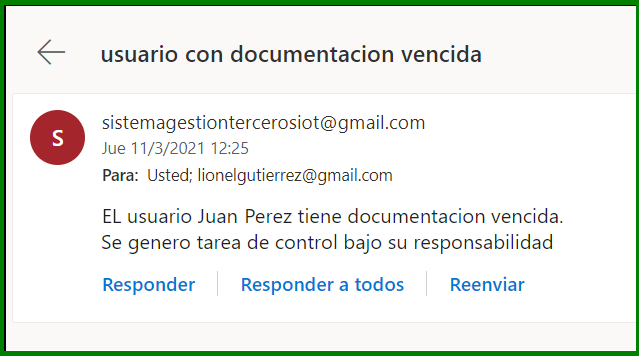
\includegraphics[width=1\textwidth]{./Figures/email.png}
	\caption{Email recibido por el usuario con la alerta de intento de ingreso con documentación vencida.}
	\label{fig:Email}
\end{figure}

En la figura \ref{fig:Tarea} se ve el paso 3 de la prueba, donde el usuario ve la tarea generada por parte del usuario.

\begin{figure}[ht]
	\centering
	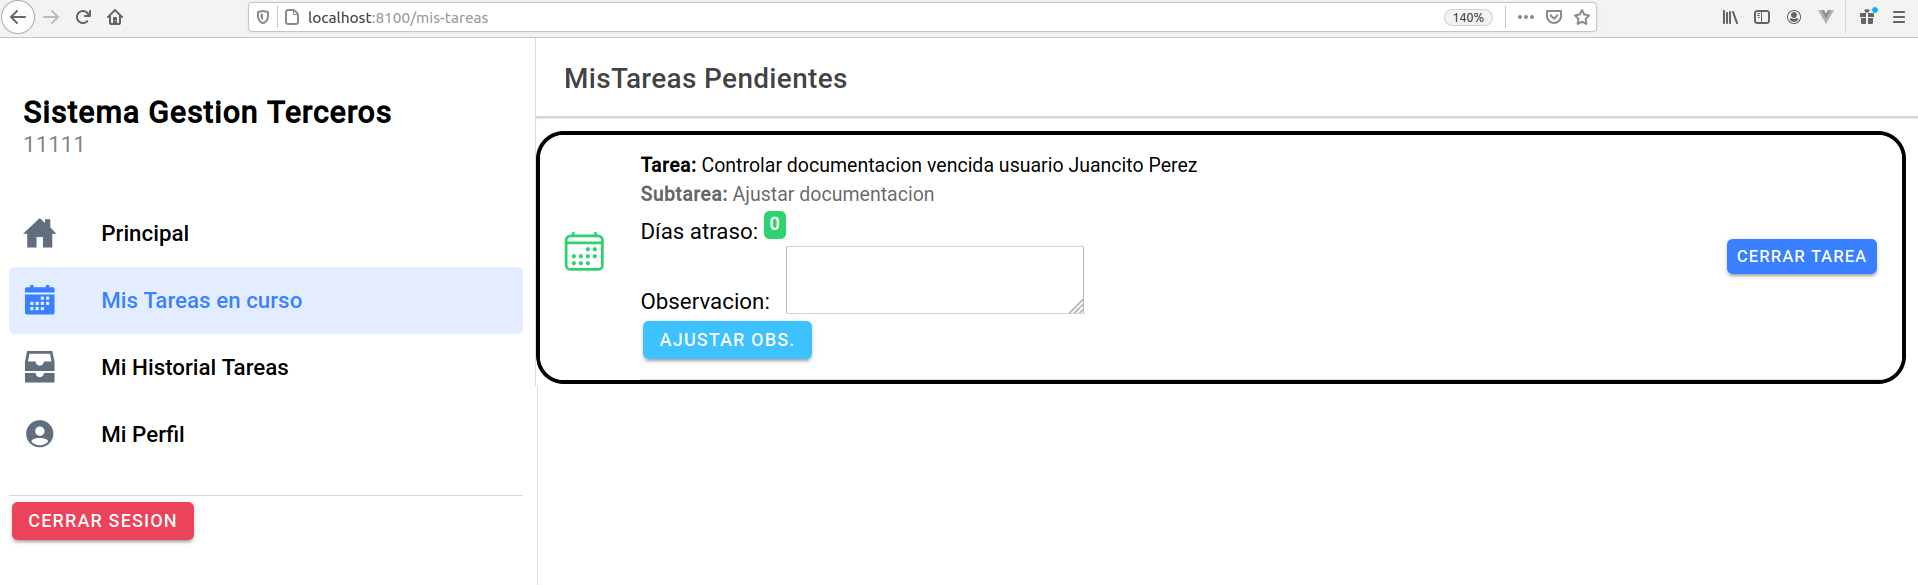
\includegraphics[width=1\textwidth]{./Figures/tarea.png}
	\caption{Pantalla de usuario se sector HESA con la tarea de control generada.}
	\label{fig:Tarea}
\end{figure}

\clearpage
\section{Comparativa con otras soluciones del mercado}

A modo de conclusión de los ensayos realizados, se hace una comparativa contra soluciones similares que existen en el mercado para el control de ingreso. De acuerdo con el análisis comparativo realizado, se destaca el diferencial de este sistema al permitir comunicarse con otros sistemas de terceros y lograr una gestión integral de accesos, con capacidad de generar alertas y tareas de control sobre el proceso.

En la tabla \ref{tab:comparacionfinal} se muestra la comparación entre el sistema implementado y soluciones similares del mercado, en la que se puede apreciar el diferencial del sistema desarrollado.


\begin{table}[h]
	\centering
	\caption[Comparación soluciones]{Comparación contra otras soluciones similares del mercado.}
	\begin{tabular}{l c c c}   
		\toprule
		\textbf{Característica} & 
		\textbf{Sistema } & 
		\textbf{Pronext KY800} &	
		\textbf{Samsung H505}    
		\\
		\midrule
		Log de ingresos  & Si  & Si & No \\		
		Interfaz a sistemas externos & Si & No & No \\		
		Gestión integral de accesos & Si & No & No \\		
		Máximo usuarios & Indefinido & 500  & 30  \\		
		Conectividad/Protocolos & Wi-Fi & Bluetooth & No  \\		
		Doble factor autenticación & No  & No & Si \\
		Tarjetas RFID  & Si  & Si  & Si \\
		Alerta de acceso  & Si & Si & Si \\
		Acceso con huella & No & Si & No \\
		\bottomrule
		\hline
	\end{tabular}
	\label{tab:comparacionfinal}
\end{table} 
% Chapter Template

\chapter{Conclusiones} % Main chapter title

\label{Chapter5} % Change X to a consecutive number; for referencing this chapter elsewhere, use \ref{ChapterX}


%----------------------------------------------------------------------------------------

%----------------------------------------------------------------------------------------
%	SECTION 1
%----------------------------------------------------------------------------------------

\section{Resultados obtenidos}

Se logró cumplir el alcance y objetivo del proyecto. En primer lugar, se implementó el sistema de control solicitado, incluyendo los módulos de sensado y actuación y la aplicación web de gestión de control y alertas. En segundo lugar, se sentaron las bases para el agregado de futuros casos de uso, para lo cual se hizo un diseño modular. Esto permitirá al sistema el sensado de datos de nuevos procesos de planta, según el requerimiento 1.1, especificado en la sección 2.5.

Adicionalmente, se pudo incorporar al sistema un módulo para gestionar la autenticación y autorización de los usuarios y el acceso a la API Rest del Backend del sistema de modo seguro. Esto posibilitó cumplir con el requerimiento 1.6, que fue agregado al trabajo durante su desarrollo. Este requerimiento permite independizar al sistema desarrollado del sistema de autenticación de la empresa y lograr una mayor portabilidad, lo que da la posibilidad a futuro de expandir el mismo a otras empresas.

Finalmente, el trabajo cumplió con el requerimiento de lograr una gestión efectiva de los terceros con un control rígido para su acceso, al sistematizar la gestión del acondicionamiento de la documentación. Si bien existen otros sistemas de control de ingreso en el mercado, se logró agregar valor mediante la comunicación del sistema en cuestión con el sistema de control de documentación de terceros y con los procesos de alerta y gestión implementados. El trabajo realizado habilita una gestión proactiva, rápida y ordenada de los terceros, de forma de actuar inmediatamente ante problemas de ingresos. Las ventajas obtenidas incluyen:

\begin{itemize}
\item Reducir tiempo para la gestión.
\item Evitar atrasos en ingresos por falta de ajustes en la documentación.
\item Evitar problemas legales ante incidentes del personal externo.
\item Evitar el uso de papel y herramientas des-centralizadas para el control y gestión de los terceros por parte de cada sector de la empresa. 
\end{itemize}

Si bien todavía el sistema no se implementó en operativo, con las pruebas realizadas y analizando los ingresos de personal en los últimos dos años, se prevé evitar un 5\% de ingresos incorrectos o con problemas, y reducir los tiempos ante inconvenientes con la documentación en unas 10 horas hombre/mes.

En la tabla \ref{tab:comparacionfinal} se muestra la comparación entre el sistema implementado y soluciones similares del mercado, en la que se puede apreciar el diferencial del sistema desarrollado.


\begin{table}[h]
	\centering
	\caption[Comparación soluciones]{Comparación contra otras soluciones similares del mercado.}
	\begin{tabular}{l c c c}   
		\toprule
		\textbf{Característica} & 
		\textbf{Sistema } & 
		\textbf{Pronext KY800} &	
		\textbf{Samsung H505}    
		\\
		\midrule
		Log de ingresos  & Si  & Si & No \\		
		Interfaz a sistemas externos & Si & No & No \\		
		Gestión integral de accesos & Si & No & No \\		
		Máximo usuarios & Indefinido & 500  & 30  \\		
		Conectividad/Protocolos & Wi-Fi & Bluetooth & No  \\		
		Doble factor autenticación & No  & No & Si \\
		Tarjetas RFID  & Si  & Si  & Si \\
		Alerta de acceso  & Si & Si & Si \\
		Acceso con huella & No & Si & No \\
		\bottomrule
		\hline
	\end{tabular}
	\label{tab:comparacionfinal}
\end{table}

Cabe destacar la importancia de los conocimientos obtenidos a lo largo de la carrera. En primer lugar, fueron muy importantes los aportes de la asignatura de gestión de proyectos. Una buena gestión de proyectos fue fundamental, tanto para lograr una planificación clara que actúe como guía a lo largo de todo el desarrollo, como para minimizar riesgos. En lo particular del trabajo, luego del comienzo del desarrollo se agregó un nuevo requerimiento al mismo. Teniendo el diagrama de Gantt \citep{WEBSITE:DiagGantt} armado, y en función del nuevo requerimiento y el avance real al momento de la solicitud, se pudo estimar el esfuerzo necesario y determinar que se podía incluir en el plan, dado que los plazos eran suficientes para poder cumplir con la fecha de finalización. Sin una gestión de proyectos clara, es muy probable que este nuevo requerimiento haya sido rechazado. 

Adicionalmente, los conocimientos en desarrollo de aplicaciones multiplataforma permitieron plantear una solución que sea \textit{web responsive} y que a futuro se puede implementar en un entorno mobile con mínimo esfuerzo. También se abre la posibilidad de implementar el sistema en la nube.

Por último, es importante mencionar que no se cumplió ninguno de los riesgos identificados durante la planificación, con lo cual no fue necesario aplicar el plan de mitigación. No obstante, el análisis y planificación temprana de los riesgos fue fundamental para hacer un seguimiento periódico, evitando que los mismos sucedan. Sin una correcta gestión y planificación, varios de los riesgos se podrían haber vuelto severos, impactando en los tiempos y recursos necesarios para completar el trabajo a término.


%----------------------------------------------------------------------------------------
%	SECTION 2
%----------------------------------------------------------------------------------------
\section{Trabajo futuro}

Para la continuidad y mejora de este trabajo se plantean dos líneas de acción.

En primer lugar, una línea de mejora del trabajo actual dentro de la que se incluyen:

\begin{itemize}
\item Realizar mejoras en seguridad:

   \begin{itemize}
      \item Agregar comunicación HTTPS entre los diferentes módulos del sistema. De este modo, se asegura que la información viaje encriptada y se evitan ataques del tipo \textit{man in the middle}. Esto permitirá migrar el sistema a la nube, donde las comunicaciones viajan entren varios sistemas abiertos, a través de Internet, y no quedan confinados al ámbito de una red interna o Intranet de una empresa.
      \item Agregar un segundo factor de autenticación al sistema. Con el objetivo de evitar que ante pérdidas o robos de la tarjeta RFID de ingreso o duplicación de la misma un atacante pueda ingresar a planta, se plantea la posibilidad de agregar un teclado matricial de forma de requerir además de la tarjeta una clave numérica durante el proceso de ingreso.
   \end{itemize}
      
   \item Automatizar tareas de configuración: se analiza implementar una aplicación para poder configurar las acciones del sistema ante las diferentes variantes de entradas (ingreso correcto, ingreso de usuario inactivo, ingreso con documentación vencida). Actualmente esta información se guarda y administra en una base de datos no relacional, por parte del personal de sistemas, que permite definir para cada tipo y valor de entrada un conjunto de acciones de salidas (tareas de control, alertas, emails). Se evalúa desarrollar una aplicación para que el usuario pueda configurar estas salidas y generar diferentes tipos de acción, independizándose del área de sistemas.
   \item Realizar una prueba de implementación en la nube: utilizar la nube de Azure para probar y asegurar el escalamiento de la solución. Esto permitirá incluir nuevas locaciones o plantas industriales al trabajo, ya sea dentro de la empresa actual o para ser implementado en nuevas empresas.
\end{itemize}   

En segundo lugar, en el marco del proyecto integral de gestión de alertas y procesos, el objetivo es incorporar nuevos procesos y casos de uso al sistema. De hecho, ya fue solicitado un primer caso de uso por parte del laboratorio de metrología de la empresa. El mismo implica el control de temperatura y humedad de dicho laboratorio, para asegurar que ambas variables se encuentren dentro de los límites requeridos y generar alertas en caso de desvíos para poder actuar en consecuencia, manual o automáticamente. 
 

%----------------------------------------------------------------------------------------
%	CONTENIDO DE LA MEMORIA  - APÉNDICES
%----------------------------------------------------------------------------------------

\appendix % indicativo para indicarle a LaTeX los siguientes "capítulos" son apéndices

% Incluir los apéndices de la memoria como archivos separadas desde la carpeta Appendices
% Descomentar las líneas a medida que se escriben los apéndices

%\include{Appendices/AppendixA}
%\include{Appendices/AppendixB}
%\include{Appendices/AppendixC}

%----------------------------------------------------------------------------------------
%	BIBLIOGRAPHY
%----------------------------------------------------------------------------------------

\Urlmuskip=0mu plus 1mu\relax
\raggedright
\printbibliography[heading=bibintoc]

%----------------------------------------------------------------------------------------

\end{document}  
